\documentclass[screen,acmsmall]{acmart}%\settopmatter{printfolios=false,printccs=false,printacmref=false}
\setcopyright{none}
\renewcommand\footnotetextcopyrightpermission[1]{}
\pagestyle{plain}

\bibliographystyle{ACM-Reference-Format}
\citestyle{acmauthoryear}   %% For author/year citations
\usepackage{listings,hyperref,multirow,paralist,xspace,url,wrapfig,tikz}
\usetikzlibrary{positioning,automata,fit,shapes.geometric,backgrounds,calc}
\usepackage{tabularx}
\newcommand{\missingTag}[1]{\textcolor{red}{#1}\xspace}
\newcommand{\missingNumber}{\textcolor{red}{XX}\xspace}
\newcommand{\missingPercentage}{\textcolor{red}{XX\%}\xspace}
\newcommand{\missingTable}[1][XX]{\textcolor{red}{Table #1}\xspace}
\newcommand{\missingGraph}{\textcolor{red}{XXGraph}\xspace}

\input{tag/corpus.tex}
\input{tag/side-effects.tex}
\input{tag/package_usage_metrics.tex}
\input{tag/kaggle_usage_metrics.tex}
\input{tag/base_usage_metrics.tex}
\newcommand{\packageNbCallSitesRnd}{17.5K\xspace}
\newcommand{\packageNbCallSites}{17,483\xspace}
\newcommand{\packageMinimizedcallsitesaRnd}{4.7K\xspace}
\newcommand{\packageMinimizedcallsitesa}{4,701\xspace}
\newcommand{\packageMinimizedcallsitesbRnd}{3.6K\xspace}
\newcommand{\packageMinimizedcallsitesb}{3,627\xspace}
\newcommand{\packageMinimizedcallsitescRnd}{2.8K\xspace}
\newcommand{\packageMinimizedcallsitesc}{2,791\xspace}
\newcommand{\packageMinimizedcallsitesdRnd}{2.2K\xspace}
\newcommand{\packageMinimizedcallsitesd}{2,181\xspace}
\newcommand{\packageMinimizedcallsiteseRnd}{1.7K\xspace}
\newcommand{\packageMinimizedcallsitese}{1,708\xspace}
\newcommand{\packageMinimizedcallsitesfRnd}{1.3K\xspace}
\newcommand{\packageMinimizedcallsitesf}{1,261\xspace}
\newcommand{\packageMinimizedcallsitesgRnd}{1.2K\xspace}
\newcommand{\packageMinimizedcallsitesg}{1,184\xspace}
\newcommand{\packageMinimizedcallsiteshRnd}{1.1K\xspace}
\newcommand{\packageMinimizedcallsitesh}{1,126\xspace}
\newcommand{\packageMinimizedcallsitesiRnd}{858\xspace}
\newcommand{\packageMinimizedcallsitesi}{858\xspace}
\newcommand{\packageMinimizedcallsitesjRnd}{731\xspace}
\newcommand{\packageMinimizedcallsitesj}{731\xspace}
\newcommand{\packageMinimizedcallsiteskRnd}{437\xspace}
\newcommand{\packageMinimizedcallsitesk}{437\xspace}
\newcommand{\packageMinimizedcallsiteslRnd}{113\xspace}
\newcommand{\packageMinimizedcallsitesl}{113\xspace}
\newcommand{\packageMinimizedpropsitesa}{27\%\xspace}
\newcommand{\packageMinimizedpropsitesb}{21\%\xspace}
\newcommand{\packageMinimizedpropsitesc}{16\%\xspace}
\newcommand{\packageMinimizedpropsitesd}{12\%\xspace}
\newcommand{\packageMinimizedpropsitese}{10\%\xspace}
\newcommand{\packageMinimizedpropsitesf}{7\%\xspace}
\newcommand{\packageMinimizedpropsitesg}{7\%\xspace}
\newcommand{\packageMinimizedpropsitesh}{6\%\xspace}
\newcommand{\packageMinimizedpropsitesi}{5\%\xspace}
\newcommand{\packageMinimizedpropsitesj}{4\%\xspace}
\newcommand{\packageMinimizedpropsitesk}{2\%\xspace}
\newcommand{\packageMinimizedpropsitesl}{0.6\%\xspace}
\newcommand{\packageMinimizedpackageaRnd}{1K\xspace}
\newcommand{\packageMinimizedpackagea}{1,012\xspace}
\newcommand{\packageMinimizedpackagebRnd}{831\xspace}
\newcommand{\packageMinimizedpackageb}{831\xspace}
\newcommand{\packageMinimizedpackagecRnd}{786\xspace}
\newcommand{\packageMinimizedpackagec}{786\xspace}
\newcommand{\packageMinimizedpackagedRnd}{768\xspace}
\newcommand{\packageMinimizedpackaged}{768\xspace}
\newcommand{\packageMinimizedpackageeRnd}{514\xspace}
\newcommand{\packageMinimizedpackagee}{514\xspace}
\newcommand{\packageMinimizedpackagefRnd}{508\xspace}
\newcommand{\packageMinimizedpackagef}{508\xspace}
\newcommand{\packageMinimizedpackagegRnd}{486\xspace}
\newcommand{\packageMinimizedpackageg}{486\xspace}
\newcommand{\packageMinimizedpackagehRnd}{129\xspace}
\newcommand{\packageMinimizedpackageh}{129\xspace}
\newcommand{\packageMinimizedpackageiRnd}{274\xspace}
\newcommand{\packageMinimizedpackagei}{274\xspace}
\newcommand{\packageMinimizedpackagejRnd}{150\xspace}
\newcommand{\packageMinimizedpackagej}{150\xspace}
\newcommand{\packageMinimizedpackagekRnd}{145\xspace}
\newcommand{\packageMinimizedpackagek}{145\xspace}
\newcommand{\packageMinimizedpackagelRnd}{67\xspace}
\newcommand{\packageMinimizedpackagel}{67\xspace}
\newcommand{\packageMinimizedoperationsaRnd}{1.2K\xspace}
\newcommand{\packageMinimizedoperationsa}{1,193\xspace}
\newcommand{\packageMinimizedoperationsbRnd}{28.3K\xspace}
\newcommand{\packageMinimizedoperationsb}{28,347\xspace}
\newcommand{\packageMinimizedoperationscRnd}{927\xspace}
\newcommand{\packageMinimizedoperationsc}{927\xspace}
\newcommand{\packageMinimizedoperationsdRnd}{5.4K\xspace}
\newcommand{\packageMinimizedoperationsd}{5,355\xspace}
\newcommand{\packageMinimizedoperationseRnd}{654\xspace}
\newcommand{\packageMinimizedoperationse}{654\xspace}
\newcommand{\packageMinimizedoperationsfRnd}{3.2K\xspace}
\newcommand{\packageMinimizedoperationsf}{3,239\xspace}
\newcommand{\packageMinimizedoperationsgRnd}{1.7K\xspace}
\newcommand{\packageMinimizedoperationsg}{1,674\xspace}
\newcommand{\packageMinimizedoperationshRnd}{56\xspace}
\newcommand{\packageMinimizedoperationsh}{56\xspace}
\newcommand{\packageMinimizedoperationsiRnd}{6.8K\xspace}
\newcommand{\packageMinimizedoperationsi}{6,830\xspace}
\newcommand{\packageMinimizedoperationsjRnd}{248.2K\xspace}
\newcommand{\packageMinimizedoperationsj}{248,166\xspace}
\newcommand{\packageMinimizedoperationskRnd}{15.2K\xspace}
\newcommand{\packageMinimizedoperationsk}{15,230\xspace}
\newcommand{\packageMinimizedoperationslRnd}{96.9K\xspace}
\newcommand{\packageMinimizedoperationsl}{96,867\xspace}
\newcommand{\packageMinimizedmedianoperationsaRnd}{5\xspace}
\newcommand{\packageMinimizedmedianoperationsa}{5\xspace}
\newcommand{\packageMinimizedmedianoperationsbRnd}{81\xspace}
\newcommand{\packageMinimizedmedianoperationsb}{81\xspace}
\newcommand{\packageMinimizedmedianoperationscRnd}{2\xspace}
\newcommand{\packageMinimizedmedianoperationsc}{2\xspace}
\newcommand{\packageMinimizedmedianoperationsdRnd}{16\xspace}
\newcommand{\packageMinimizedmedianoperationsd}{16\xspace}
\newcommand{\packageMinimizedmedianoperationseRnd}{8\xspace}
\newcommand{\packageMinimizedmedianoperationse}{8\xspace}
\newcommand{\packageMinimizedmedianoperationsfRnd}{1.9K\xspace}
\newcommand{\packageMinimizedmedianoperationsf}{1,929\xspace}
\newcommand{\packageMinimizedmedianoperationsgRnd}{95\xspace}
\newcommand{\packageMinimizedmedianoperationsg}{95\xspace}
\newcommand{\packageMinimizedmedianoperationshRnd}{10\xspace}
\newcommand{\packageMinimizedmedianoperationsh}{10\xspace}
\newcommand{\packageMinimizedmedianoperationsiRnd}{60\xspace}
\newcommand{\packageMinimizedmedianoperationsi}{60\xspace}
\newcommand{\packageMinimizedmedianoperationsjRnd}{5K\xspace}
\newcommand{\packageMinimizedmedianoperationsj}{4,967.5\xspace}
\newcommand{\packageMinimizedmedianoperationskRnd}{70\xspace}
\newcommand{\packageMinimizedmedianoperationsk}{70\xspace}
\newcommand{\packageMinimizedmedianoperationslRnd}{11.6K\xspace}
\newcommand{\packageMinimizedmedianoperationsl}{11,642\xspace}
\newcommand{\packageMinimizedpercentenvira}{73\%\xspace}
\newcommand{\packageMinimizedpercentenvirb}{61\%\xspace}
\newcommand{\packageMinimizedpercentenvirc}{62\%\xspace}
\newcommand{\packageMinimizedpercentenvird}{56\%\xspace}
\newcommand{\packageMinimizedpercentenvire}{47\%\xspace}
\newcommand{\packageMinimizedpercentenvirf}{80\%\xspace}
\newcommand{\packageMinimizedpercentenvirg}{45\%\xspace}
\newcommand{\packageMinimizedpercentenvirh}{82\%\xspace}
\newcommand{\packageMinimizedpercentenviri}{24\%\xspace}
\newcommand{\packageMinimizedpercentenvirj}{44\%\xspace}
\newcommand{\packageMinimizedpercentenvirk}{35\%\xspace}
\newcommand{\packageMinimizedpercentenvirl}{47\%\xspace}
\newcommand{\packageMinimizedpercentcallsenvira}{81\%\xspace}
\newcommand{\packageMinimizedpercentcallsenvirb}{47\%\xspace}
\newcommand{\packageMinimizedpercentcallsenvirc}{59\%\xspace}
\newcommand{\packageMinimizedpercentcallsenvird}{68\%\xspace}
\newcommand{\packageMinimizedpercentcallsenvire}{60\%\xspace}
\newcommand{\packageMinimizedpercentcallsenvirf}{72\%\xspace}
\newcommand{\packageMinimizedpercentcallsenvirg}{19\%\xspace}
\newcommand{\packageMinimizedpercentcallsenvirh}{18\%\xspace}
\newcommand{\packageMinimizedpercentcallsenviri}{8\%\xspace}
\newcommand{\packageMinimizedpercentcallsenvirj}{74\%\xspace}
\newcommand{\packageMinimizedpercentcallsenvirk}{10\%\xspace}
\newcommand{\packageMinimizedpercentcallsenvirl}{21\%\xspace}
\newcommand{\packageMinimizedpercentenvirnonparenta}{55\%\xspace}
\newcommand{\packageMinimizedpercentenvirnonparentb}{21\%\xspace}
\newcommand{\packageMinimizedpercentenvirnonparentc}{37\%\xspace}
\newcommand{\packageMinimizedpercentenvirnonparentd}{37\%\xspace}
\newcommand{\packageMinimizedpercentenvirnonparente}{28\%\xspace}
\newcommand{\packageMinimizedpercentenvirnonparentf}{14\%\xspace}
\newcommand{\packageMinimizedpercentenvirnonparentg}{28\%\xspace}
\newcommand{\packageMinimizedpercentenvirnonparenth}{6\%\xspace}
\newcommand{\packageMinimizedpercentenvirnonparenti}{21\%\xspace}
\newcommand{\packageMinimizedpercentenvirnonparentj}{19\%\xspace}
\newcommand{\packageMinimizedpercentenvirnonparentk}{13\%\xspace}
\newcommand{\packageMinimizedpercentenvirnonparentl}{38\%\xspace}
\newcommand{\packageMinimizedpercentparentframesa}{48\%\xspace}
\newcommand{\packageMinimizedpercentparentframesb}{79\%\xspace}
\newcommand{\packageMinimizedpercentparentframesc}{71\%\xspace}
\newcommand{\packageMinimizedpercentparentframesd}{68\%\xspace}
\newcommand{\packageMinimizedpercentparentframese}{79\%\xspace}
\newcommand{\packageMinimizedpercentparentframesf}{46\%\xspace}
\newcommand{\packageMinimizedpercentparentframesg}{77\%\xspace}
\newcommand{\packageMinimizedpercentparentframesh}{96\%\xspace}
\newcommand{\packageMinimizedpercentparentframesi}{78\%\xspace}
\newcommand{\packageMinimizedpercentparentframesj}{84\%\xspace}
\newcommand{\packageMinimizedpercentparentframesk}{87\%\xspace}
\newcommand{\packageMinimizedpercentparentframesl}{79\%\xspace}
\newcommand{\packageNbSimpleMinimizedOneRnd}{7.2K\xspace}
\newcommand{\packageNbSimpleMinimizedOne}{7,217\xspace}
\newcommand{\packageNbSimpleMinimizedMoreRnd}{601\xspace}
\newcommand{\packageNbSimpleMinimizedMore}{601\xspace}
\newcommand{\packageNbSymbolVarSitesRnd}{2.3K\xspace}
\newcommand{\packageNbSymbolVarSites}{2,349\xspace}
\newcommand{\packageNbSymbolVarSitePercent}{50\%\xspace}
\newcommand{\packageNbNonDefaultEnvirVariablesPercent}{82.5\%\xspace}
\newcommand{\packageFunctionDefinitionSitesRnd}{1.1K\xspace}
\newcommand{\packageFunctionDefinitionSites}{1,126\xspace}
\newcommand{\packageFunctionDefinitionSitesPercent}{6.4\%\xspace}
\newcommand{\packageFundefNonDefaultEnvirSitesPercent}{82.4\%\xspace}
\newcommand{\packageGeneralizedFunctionDefinitionSitesRnd}{1.8K\xspace}
\newcommand{\packageGeneralizedFunctionDefinitionSites}{1,753\xspace}
\newcommand{\packageGeneralizedFunctionDefinitionSitesPercent}{10\%\xspace}
\newcommand{\packageGeneralizedFundedNonDefaultEnvirSitesPercent}{52.9\%\xspace}
\newcommand{\packageNbAssignSitesRnd}{1.2K\xspace}
\newcommand{\packageNbAssignSites}{1,245\xspace}
\newcommand{\packageAssignSitesPercent}{7.1\%\xspace}
\newcommand{\packageNonDefaultEnvirAssignSitesRnd}{339\xspace}
\newcommand{\packageNonDefaultEnvirAssignSites}{339\xspace}
\newcommand{\packageNonDefaultEnvirAssignSitesPercent}{27.2\%\xspace}
\newcommand{\packageNbOneMinimizedRnd}{15.3K\xspace}
\newcommand{\packageNbOneMinimized}{15,307\xspace}
\newcommand{\packageNbOneMinimizedPercent}{87.6\%\xspace}
\newcommand{\packageNbCallSitesUniqueActualValueRnd}{1.4K\xspace}
\newcommand{\packageNbCallSitesUniqueActualValue}{1,436\xspace}
\newcommand{\packageCallSitesUniqueActualValuePercent}{51.5\%\xspace}
\newcommand{\packageMedianRunSitesUniqueActualValueRnd}{2\xspace}
\newcommand{\packageMedianRunSitesUniqueActualValue}{2\xspace}
\newcommand{\packageAverageRunSitesUniqueActualValueRnd}{14\xspace}
\newcommand{\packageAverageRunSitesUniqueActualValue}{14\xspace}
\newcommand{\packageSdRunSitesUniqueActualValueRnd}{57.9\xspace}
\newcommand{\packageSdRunSitesUniqueActualValue}{57.9\xspace}
\newcommand{\packageValOneNodeRnd}{2.2K\xspace}
\newcommand{\packageValOneNode}{2,228\xspace}
\newcommand{\packageValOneNodePercent}{74.6\%\xspace}
\newcommand{\packageOneValMedianRunsRnd}{2\xspace}
\newcommand{\packageOneValMedianRuns}{2\xspace}
\newcommand{\packageOneValAverageRunsRnd}{32.7\xspace}
\newcommand{\packageOneValAverageRuns}{32.7\xspace}
\newcommand{\packageOneValSdRunsRnd}{695\xspace}
\newcommand{\packageOneValSdRuns}{695\xspace}
\newcommand{\packageNonDefaultEnvirValuePercent}{64.1\%\xspace}
\newcommand{\packageNonDefaultEnvirWithVarPercent}{34.7\%\xspace}
\newcommand{\packageNbSlotAccessRnd}{1.7K\xspace}
\newcommand{\packageNbSlotAccess}{1,708\xspace}
\newcommand{\packageSlotAccessPercent}{9.8\%\xspace}
\newcommand{\packageGeneralizedSlotAccessRnd}{3K\xspace}
\newcommand{\packageGeneralizedSlotAccess}{3,019\xspace}
\newcommand{\packageGeneralizedSlotAccessPercent}{17.3\%\xspace}
\newcommand{\packageNdefaultEnvirSlotSiteRnd}{1.3K\xspace}
\newcommand{\packageNdefaultEnvirSlotSite}{1,306\xspace}
\newcommand{\packageNdefaultEnvirSlotSitePercent}{43.3\%\xspace}
\newcommand{\packageGeneralizedVarAccessSitesRnd}{7.6K\xspace}
\newcommand{\packageGeneralizedVarAccessSites}{7,635\xspace}
\newcommand{\packageGeneralizedVarAccessSitePercent}{43.7\%\xspace}

\input{tag/kaggle_normalized_expr.tex}
\input{tag/base_normalized_expr.tex}
\input{tag/package_environments.tex}
%\input{tag/package_provenance.tex}
\newcommand{\packageNbProvenanceCallsaRnd}{23.5M\xspace}
\newcommand{\packageNbProvenanceCallsa}{23,478,269\xspace}
\newcommand{\packageNbProvenanceCallsbRnd}{8.5M\xspace}
\newcommand{\packageNbProvenanceCallsb}{8,458,959\xspace}
\newcommand{\packageNbProvenanceCallscRnd}{3M\xspace}
\newcommand{\packageNbProvenanceCallsc}{3,042,180\xspace}
\newcommand{\packageNbProvenanceCallsdRnd}{2.3M\xspace}
\newcommand{\packageNbProvenanceCallsd}{2,318,201\xspace}
\newcommand{\packageNbProvenanceCallseRnd}{1.4M\xspace}
\newcommand{\packageNbProvenanceCallse}{1,359,948\xspace}
\newcommand{\packageNbProvenanceCallsfRnd}{1.1M\xspace}
\newcommand{\packageNbProvenanceCallsf}{1,141,083\xspace}
\newcommand{\packageNbProvenanceCallsgRnd}{704.9K\xspace}
\newcommand{\packageNbProvenanceCallsg}{704,853\xspace}
\newcommand{\packageNbProvenanceCallshRnd}{647.3K\xspace}
\newcommand{\packageNbProvenanceCallsh}{647,295\xspace}
\newcommand{\packageNbProvenanceCallsiRnd}{543.8K\xspace}
\newcommand{\packageNbProvenanceCallsi}{543,759\xspace}
\newcommand{\packageNbProvenanceCallsjRnd}{542.6K\xspace}
\newcommand{\packageNbProvenanceCallsj}{542,581\xspace}
\newcommand{\packagePercentProvenanceCallsaRnd}{53.9\xspace}
\newcommand{\packagePercentProvenanceCallsa}{53.9\xspace}
\newcommand{\packagePercentProvenanceCallsbRnd}{19.4\xspace}
\newcommand{\packagePercentProvenanceCallsb}{19.4\xspace}
\newcommand{\packagePercentProvenanceCallscRnd}{7\xspace}
\newcommand{\packagePercentProvenanceCallsc}{7\xspace}
\newcommand{\packagePercentProvenanceCallsdRnd}{5.3\xspace}
\newcommand{\packagePercentProvenanceCallsd}{5.3\xspace}
\newcommand{\packagePercentProvenanceCallseRnd}{3.1\xspace}
\newcommand{\packagePercentProvenanceCallse}{3.1\xspace}
\newcommand{\packagePercentProvenanceCallsfRnd}{2.6\xspace}
\newcommand{\packagePercentProvenanceCallsf}{2.6\xspace}
\newcommand{\packagePercentProvenanceCallsgRnd}{1.6\xspace}
\newcommand{\packagePercentProvenanceCallsg}{1.6\xspace}
\newcommand{\packagePercentProvenanceCallshRnd}{1.5\xspace}
\newcommand{\packagePercentProvenanceCallsh}{1.5\xspace}
\newcommand{\packagePercentProvenanceCallsiRnd}{1.2\xspace}
\newcommand{\packagePercentProvenanceCallsi}{1.2\xspace}
\newcommand{\packagePercentProvenanceCallsjRnd}{1.2\xspace}
\newcommand{\packagePercentProvenanceCallsj}{1.2\xspace}
\newcommand{\packageCumpercentProvenanceCallsaRnd}{53.9\xspace}
\newcommand{\packageCumpercentProvenanceCallsa}{53.9\xspace}
\newcommand{\packageCumpercentProvenanceCallsbRnd}{73.4\xspace}
\newcommand{\packageCumpercentProvenanceCallsb}{73.4\xspace}
\newcommand{\packageCumpercentProvenanceCallscRnd}{80.4\xspace}
\newcommand{\packageCumpercentProvenanceCallsc}{80.4\xspace}
\newcommand{\packageCumpercentProvenanceCallsdRnd}{85.7\xspace}
\newcommand{\packageCumpercentProvenanceCallsd}{85.7\xspace}
\newcommand{\packageCumpercentProvenanceCallseRnd}{88.8\xspace}
\newcommand{\packageCumpercentProvenanceCallse}{88.8\xspace}
\newcommand{\packageCumpercentProvenanceCallsfRnd}{91.4\xspace}
\newcommand{\packageCumpercentProvenanceCallsf}{91.4\xspace}
\newcommand{\packageCumpercentProvenanceCallsgRnd}{93.1\xspace}
\newcommand{\packageCumpercentProvenanceCallsg}{93.1\xspace}
\newcommand{\packageCumpercentProvenanceCallshRnd}{94.5\xspace}
\newcommand{\packageCumpercentProvenanceCallsh}{94.5\xspace}
\newcommand{\packageCumpercentProvenanceCallsiRnd}{95.8\xspace}
\newcommand{\packageCumpercentProvenanceCallsi}{95.8\xspace}
\newcommand{\packageCumpercentProvenanceCallsjRnd}{97\xspace}
\newcommand{\packageCumpercentProvenanceCallsj}{97\xspace}
\newcommand{\packageProvenanceNamea}{parse\xspace}
\newcommand{\packageProvenanceNameb}{substitute\xspace}
\newcommand{\packageProvenanceNamec}{match.call\xspace}
\newcommand{\packageProvenanceNamed}{NA\xspace}
\newcommand{\packageProvenanceNamee}{expression\xspace}
\newcommand{\packageProvenanceNamef}{quote\xspace}
\newcommand{\packageProvenanceNameg}{as.name\xspace}
\newcommand{\packageProvenanceNameh}{call\xspace}
\newcommand{\packageProvenanceNamei}{as.call\xspace}
\newcommand{\packageProvenanceNamej}{[[\xspace}
\newcommand{\packageProvenanceNamek}{\$\xspace}
\newcommand{\packageProvenanceNamel}{.External\xspace}
\newcommand{\packageProvenanceNamem}{as.vector\xspace}
\newcommand{\packageProvenanceNamen}{formals\xspace}
\newcommand{\packageNbProvenanceSitesaRnd}{4K\xspace}
\newcommand{\packageNbProvenanceSitesa}{4,006\xspace}
\newcommand{\packageNbProvenanceSitesbRnd}{3.9K\xspace}
\newcommand{\packageNbProvenanceSitesb}{3,916\xspace}
\newcommand{\packageNbProvenanceSitescRnd}{2.1K\xspace}
\newcommand{\packageNbProvenanceSitesc}{2,058\xspace}
\newcommand{\packageNbProvenanceSitesdRnd}{1.1K\xspace}
\newcommand{\packageNbProvenanceSitesd}{1,116\xspace}
\newcommand{\packageNbProvenanceSiteseRnd}{597\xspace}
\newcommand{\packageNbProvenanceSitese}{597\xspace}
\newcommand{\packageNbProvenanceSitesfRnd}{557\xspace}
\newcommand{\packageNbProvenanceSitesf}{557\xspace}
\newcommand{\packageNbProvenanceSitesgRnd}{482\xspace}
\newcommand{\packageNbProvenanceSitesg}{482\xspace}
\newcommand{\packageNbProvenanceSiteshRnd}{475\xspace}
\newcommand{\packageNbProvenanceSitesh}{475\xspace}
\newcommand{\packageNbProvenanceSitesiRnd}{450\xspace}
\newcommand{\packageNbProvenanceSitesi}{450\xspace}
\newcommand{\packageNbProvenanceSitesjRnd}{364\xspace}
\newcommand{\packageNbProvenanceSitesj}{364\xspace}
\newcommand{\packageNbProvenanceSiteskRnd}{271\xspace}
\newcommand{\packageNbProvenanceSitesk}{271\xspace}
\newcommand{\packageNbProvenanceSiteslRnd}{251\xspace}
\newcommand{\packageNbProvenanceSitesl}{251\xspace}
\newcommand{\packageNbProvenanceSitesmRnd}{210\xspace}
\newcommand{\packageNbProvenanceSitesm}{210\xspace}
\newcommand{\packageNbProvenanceSitesnRnd}{112\xspace}
\newcommand{\packageNbProvenanceSitesn}{112\xspace}
\newcommand{\packagePercentProvenanceSitesaRnd}{22.9\xspace}
\newcommand{\packagePercentProvenanceSitesa}{22.9\xspace}
\newcommand{\packagePercentProvenanceSitesbRnd}{22.4\xspace}
\newcommand{\packagePercentProvenanceSitesb}{22.4\xspace}
\newcommand{\packagePercentProvenanceSitescRnd}{11.8\xspace}
\newcommand{\packagePercentProvenanceSitesc}{11.8\xspace}
\newcommand{\packagePercentProvenanceSitesdRnd}{6.4\xspace}
\newcommand{\packagePercentProvenanceSitesd}{6.4\xspace}
\newcommand{\packagePercentProvenanceSiteseRnd}{3.4\xspace}
\newcommand{\packagePercentProvenanceSitese}{3.4\xspace}
\newcommand{\packagePercentProvenanceSitesfRnd}{3.2\xspace}
\newcommand{\packagePercentProvenanceSitesf}{3.2\xspace}
\newcommand{\packagePercentProvenanceSitesgRnd}{2.8\xspace}
\newcommand{\packagePercentProvenanceSitesg}{2.8\xspace}
\newcommand{\packagePercentProvenanceSiteshRnd}{2.7\xspace}
\newcommand{\packagePercentProvenanceSitesh}{2.7\xspace}
\newcommand{\packagePercentProvenanceSitesiRnd}{2.6\xspace}
\newcommand{\packagePercentProvenanceSitesi}{2.6\xspace}
\newcommand{\packagePercentProvenanceSitesjRnd}{2.1\xspace}
\newcommand{\packagePercentProvenanceSitesj}{2.1\xspace}
\newcommand{\packagePercentProvenanceSiteskRnd}{1.6\xspace}
\newcommand{\packagePercentProvenanceSitesk}{1.6\xspace}
\newcommand{\packagePercentProvenanceSiteslRnd}{1.4\xspace}
\newcommand{\packagePercentProvenanceSitesl}{1.4\xspace}
\newcommand{\packagePercentProvenanceSitesmRnd}{1.2\xspace}
\newcommand{\packagePercentProvenanceSitesm}{1.2\xspace}
\newcommand{\packagePercentProvenanceSitesnRnd}{0.6\xspace}
\newcommand{\packagePercentProvenanceSitesn}{0.6\xspace}
\newcommand{\packageCumpercentProvenanceSitesaRnd}{22.9\xspace}
\newcommand{\packageCumpercentProvenanceSitesa}{22.9\xspace}
\newcommand{\packageCumpercentProvenanceSitesbRnd}{45.3\xspace}
\newcommand{\packageCumpercentProvenanceSitesb}{45.3\xspace}
\newcommand{\packageCumpercentProvenanceSitescRnd}{57.1\xspace}
\newcommand{\packageCumpercentProvenanceSitesc}{57.1\xspace}
\newcommand{\packageCumpercentProvenanceSitesdRnd}{63.5\xspace}
\newcommand{\packageCumpercentProvenanceSitesd}{63.5\xspace}
\newcommand{\packageCumpercentProvenanceSiteseRnd}{66.9\xspace}
\newcommand{\packageCumpercentProvenanceSitese}{66.9\xspace}
\newcommand{\packageCumpercentProvenanceSitesfRnd}{70.1\xspace}
\newcommand{\packageCumpercentProvenanceSitesf}{70.1\xspace}
\newcommand{\packageCumpercentProvenanceSitesgRnd}{72.8\xspace}
\newcommand{\packageCumpercentProvenanceSitesg}{72.8\xspace}
\newcommand{\packageCumpercentProvenanceSiteshRnd}{75.5\xspace}
\newcommand{\packageCumpercentProvenanceSitesh}{75.5\xspace}
\newcommand{\packageCumpercentProvenanceSitesiRnd}{78.1\xspace}
\newcommand{\packageCumpercentProvenanceSitesi}{78.1\xspace}
\newcommand{\packageCumpercentProvenanceSitesjRnd}{80.2\xspace}
\newcommand{\packageCumpercentProvenanceSitesj}{80.2\xspace}
\newcommand{\packageCumpercentProvenanceSiteskRnd}{81.7\xspace}
\newcommand{\packageCumpercentProvenanceSitesk}{81.7\xspace}
\newcommand{\packageCumpercentProvenanceSiteslRnd}{83.2\xspace}
\newcommand{\packageCumpercentProvenanceSitesl}{83.2\xspace}
\newcommand{\packageCumpercentProvenanceSitesmRnd}{84.4\xspace}
\newcommand{\packageCumpercentProvenanceSitesm}{84.4\xspace}
\newcommand{\packageCumpercentProvenanceSitesnRnd}{85\xspace}
\newcommand{\packageCumpercentProvenanceSitesn}{85\xspace}
\newcommand{\packageNbStringSitesRnd}{4.1K\xspace}
\newcommand{\packageNbStringSites}{4,107\xspace}
\newcommand{\packageStringSitesPercent}{23.5\%\xspace}
\newcommand{\packageNbReflectionSitesRnd}{7.9K\xspace}
\newcommand{\packageNbReflectionSites}{7,857\xspace}
\newcommand{\packageReflectionSitesPercent}{44.9\%\xspace}
\newcommand{\packageNbConstructedSitesRnd}{3.1K\xspace}
\newcommand{\packageNbConstructedSites}{3,086\xspace}
\newcommand{\packageConstructedSitesPercent}{17.7\%\xspace}
\newcommand{\packageNbSymbolSitesRnd}{1.2K\xspace}
\newcommand{\packageNbSymbolSites}{1,200\xspace}
\newcommand{\packageSymbolSitesPercent}{6.9\%\xspace}
\newcommand{\packageNbExternalSitesRnd}{278\xspace}
\newcommand{\packageNbExternalSites}{278\xspace}
\newcommand{\packageExternalSitesPercent}{1.6\%\xspace}
\newcommand{\packageNbParseFromFileSitesRnd}{11\xspace}
\newcommand{\packageNbParseFromFileSites}{11\xspace}

\input{tag/kaggle_provenance.tex}

\graphicspath{{img/}}

\lstset{language=R}

\definecolor{LightGray}{rgb}{.92,.92,.92}
\definecolor{Gray}{rgb}{.3,.3,.3}
\definecolor{DarkGray}{rgb}{.5,.5,.5}

\lstset{ %
  columns=flexible,
  captionpos=b,
  frame=single,
  framerule=0pt,
  framexleftmargin=-1mm,
  framexrightmargin=-1mm,
  tabsize=2,
  belowskip=0pt,
  basicstyle=\small\ttfamily,
  backgroundcolor=\color{LightGray},
  keywordstyle=\small\ttfamily\bfseries,
  commentstyle=\color{Gray}\em,
  stringstyle=\color{DarkGray}, %
  literate={<-}{{$\leftarrow$\,}}1{<<-}{{$\twoheadleftarrow$}}1,
  keywords={new, env, call, eval, evalq, function, local, parent, quote
            return, ifelse, for, in, frame, basenv},
}

\lstdefinestyle{R}{ language=R, breaklines=true }

\newcommand{\eg}{\emph{e.g.},\xspace\xspace}
\newcommand{\ie}{\emph{i.e.},\xspace}
\newcommand{\cf}{\emph{cf.}\xspace}
\newcommand{\summary}[1]{{\csname #1\endcsname} ({\csname #1Min\endcsname} / {\csname #1Mean\endcsname} / {\csname #1Max\endcsname})}
\newcommand{\summaryrnd}[1]{{\csname #1Rnd\endcsname} ({\csname #1MinRnd\endcsname} / {\csname #1MeanRnd\endcsname} / {\csname #1MaxRnd\endcsname})}

\newcommand{\eval}{\texttt{eval}\xspace}
\newcommand{\Eval}{\texttt{Eval}\xspace}
\newcommand{\evals}{{\sf eval}s\xspace}
\newcommand{\parse}{\c{parse}}
\newcommand{\source}{\c{source}}
\newcommand{\local}{\c{local}}
\newcommand{\unlockBinding}{\c{unlockBinding}}
\newcommand{\substitute}{\c{substitute}}
\newcommand{\datatable}{\c{data.table}}
\newcommand{\mlogit}{\c{mlogit}}
\newcommand{\mboost}{\c{mboost}}
\newcommand{\metafor}{\c{metafor}}
\newcommand{\lavaan}{\c{lavaan}}
\newcommand{\mclust}{\c{mclust}}
\newcommand{\gamlss}{\c{gamlss}}
\newcommand{\ggproto}{\c{ggproto}}
\newcommand{\ggplot}{\c{ggplot2}}
\newcommand{\base}{\c{base}}
\renewcommand{\c}[1]{{\sf #1}\xspace}
\newcommand{\miss}[1]{{\textcolor{red}{#1}}\xspace}
\newcommand{\evil}{\emph{evil}\xspace}
\newcommand{\instrumentr}{\emph{instrumentr}\xspace}
\newcommand{\rdyntrace}{\emph{R-dyntrace}\xspace}
\newcommand{\covr}{\emph{covr}\xspace}
\newcommand{\runr}{\emph{runr}\xspace}
\newcommand{\genthat}{\emph{genthat}\xspace}

\newcommand{\NOTE}[1]{{\it Note: #1}\xspace}
\newcommand{\authorcomment}[3]{\xspace\textcolor{#1}{{\bf #2} #3}\xspace}
\newcommand{\todo}[1]{\authorcomment{red}{TODO}{#1}}
\newcommand{\code}[1]{\lstinline |#1|\xspace}
%\renewcommand{\c}[1]{\lstinline |#1|\xspace}
% cf. https://tex.stackexchange.com/a/144640
\makeatletter\let\expandableinput\@@input\makeatother
\lstdefinelanguage{smalleR} {
  morekeywords={
    for,
    if,
    else,
    function
  },
  sensitive=true, % keywords are not case-sensitive
  morecomment=[l]{\#}, % l is for line comment
  morestring=[b]{"} % defines that strings are enclosed in double quotes
}
\lstset{
  language={smalleR},
  columns=flexible,
  captionpos=b,
  frame=single,
  framerule=0pt,
%  framexleftmargin=1mm,
%  framexrightmargin=1mm,
  tabsize=2,
  belowskip=0pt,
  basicstyle=\small\ttfamily,
  backgroundcolor=\color{LightGray},
  emphstyle=\sffamily,
  keywordstyle=\bfseries,
  commentstyle=\color{Gray}\em,
  stringstyle=\color{Gray},
  alsoletter={., _, $},
  breaklines=true
}

\begin{document}
\title{What We Eval in the Shadows}
\subtitle{A Large-scale Study of Eval in R programs}

\author{Aviral Goel}\affiliation{\institution{Northeastern
    University}\country{USA}}
\author{Pierre Donat-Bouillud}\affiliation{\institution{Czech Technical University in Prague}\country{Czech Republic}}
\author{Filip Křikava}\affiliation{\institution{Czech Technical University in Prague}\country{Czech Republic}}
\author{Christoph Kirsch}\affiliation{\institution{Czech Technical University in Prague}\country{Czech Republic}}
\author{Jan Vitek}\affiliation{\institution{Northeastern University}\country{USA}}
\affiliation{\institution{Czech Technical University in Prague}\country{Czech Republic}}

\begin{abstract}
 Most dynamic languages allow users to turn text into code using
  various functions, often named \eval, with language-dependent semantics. The
  widespread use of these reflective functions hinders static analysis and
  prevents compilers from performing optimizations. This paper aims to provide a
  better sense of why programmers use \eval. Understanding why \eval is used in
  practice is key to finding ways to mitigate its negative impact. We have
  reasons to believe that reflective feature usage is language and application
  domain-specific; we focus on data science code written in R and compare our
  results to previous work that analyzed web programming in JavaScript. This
  paper studied \CranRunnableScripts scripts extracted from \CranPackages R
  packages, for a total of \packageAllcalls calls to \eval. We find that \eval
  is indeed in widespread use; R's \eval is more pervasive and arguably
  dangerous than what was previously reported for JavaScript.
\end{abstract}

\maketitle
\renewcommand{\shortauthors}{Goel et al.}
\renewcommand{\shorttitle}{What We Eval in the Shadows}

\section{Introduction}

Most dynamic languages provide their users with a facility to transform
unstructured text into executable code and evaluate that code. We refer to this
reflective facility as \eval bowing to its origins in LISP, all the way back in
1956. \Eval has been much maligned over the years. In computing lore, it is as
close to a boogeyman as it gets. Yet, for McCarthy, \eval was simply the way to
write down the definition of LISP; he was surprised that someone coded it up and
offered it to end users~\cite{lisp}. Since then, reflective facilities have been
used to parameterize programs over code patterns that can be provided after the
program is written. The presence of such a feature in a language is a hallmark
of dynamism; it is a form of delayed binding as the behavior of any particular
call to \eval will only be known when the program is run, and that particular
call site is evaluated.

\paragraph{Trouble in Paradise.} Reflective facilities hinder
most attempts to reason about or apply meaning-preserving transformations to the
code using them. In practice, \eval causes static analysis techniques to lose so
much precision as to become pointless. For compilers, anything but the most
trivial, local optimizations are unsound after use of \eval. Furthermore, the
addition of arbitrary code --- code that could have been obtained from a network
connection --- as a program is running is a security vulnerability waiting to
happen. To illustrate these challenges, consider the interaction of a static
analysis tool with a dynamic language. A program analyzer computes an
over-approximation of the set of possible behaviors exhibited by the program
under study, a reflective facility must be represented by all behaviors that can
be expressed in the target language. \ie any legal sequence of instructions can
replace \eval. As dynamic languages are permissive, the tool must assume that
all functions in scope were redefined, \eg that \texttt{`+`} now opens a network
connection. A single occurrence of \eval causes the static analyzer to lose all
information about the program state and meaning of identifiers. This loss of
precision can sometimes be mitigated by analyzing the string
argument~\cite{moller03}, but if the string comes from outside the program, not
much can be done. A frustrated group of researchers argued giving up on
soundness and, instead, under-approximating dynamic features
(soundiness)~\cite{soundy}. In their words, ``a practical analysis, may pretend
that \eval does nothing unless it can precisely resolve its string argument at
compile time.'' Alas, assuming that \eval does not have side-effects or that
side-effects will not affect results is unduly optimistic.

\paragraph{Is Past Prologue?} Previous work investigated
\eval in web programming, specifically JavaScript web pages~\cite{pldi10a}. In
2011, 82\% of the 10,000 most accessed sites used \eval~\cite{ecoop11}. Yet, the
strings passed to \eval, and their behaviors, when executed, were far from
random; it was shown that when one could observe several calls, the ``shape'' of
future calls could be predicted with 97\% accuracy~\cite{oopsla12b}. Overall,
practical usage suggested that most reflective calls were relatively harmless.
While this backed up the soundiness squad's approach, does it generalize to
other application domains and to other languages?

\paragraph{The Here and Now.} In this study, we investigate the
usage of \eval in programs written in the R language. R is a language designed
by statisticians for applications in data science~\cite{r,R96}. What makes
looking at R after JavaScript interesting is that, while both languages are
dynamic, they are quite different. While one can program in an object-oriented
style in R like in JavaScript, R is mostly a lazy functional language.
JavaScript was designed to run untrusted code in a browser, while R is used for
statistical computing on desktops. JavaScript is a general-purpose language used
by a vast community of programmers, while R is used for scientific computing by
data scientists and domain experts with, often, limited programming experience.
One can distinguish between library implementers who have programming experience
and a working knowledge of R, and end-users who are typically not expert
programmers with a cursory knowledge of the language.\footnote{We surveyed
end-users and did not find a single one aware that R is lazy.} Our goal is to
highlight the differences in usage between JavaScript and R and explain them in
terms of language features, application domain and programmer experience.
Hopefully, some of our observations generalize to other languages. Our data
and code are open source and publicly available:
\url{https://github.com/PRL-PRG/evalr-experiment}.

\paragraph{The What and How.} One benefit of
R is that every package in the CRAN repository comes with examples of typical
usage. This gives us a codebase that we can analyze dynamically. To observe
\eval, we built a two-level monitoring infrastructure: we monitor programs by
instrumentation and we also monitor the inner workings of the interpreter.
Dynamic analysis is limited as it can only observe behaviors triggered by the
particular inputs passed to a program. Luckily, R libraries come with many tests
and use-cases. Our corpus is constructed to reflect the levels of sophistication
of the R community. We distinguish between \emph{CRAN packages} (\CranPackages
curated packages that pass quality checks and have tests and sample data) and
\emph{Kaggle scripts} (\KaggleUnique end-user written programs) It is reasonable
to expect \eval usage to differ between these datasets, libraries are part of a
lively and growing ecosystem, while end-user code is often thrown together, run
once, and never revisited.


\paragraph{Why do we Eval?} The results of our study suggest
that \eval is widely used for the implementation of the language, and in many
libraries. End-user code makes less frequent and less sophisticated use of
\eval. In many ways, \eval in R is as bad as it gets: it's varied, performs
side-effects and reaches to many environments. By large, the motivations for
\eval relate to various forms of language extensions and meta-programming. \Eval
is used where other languages would provide macros. But, the expressive power of
\eval is higher as it can reach arbitrarily far back in the call stack.


\section{Background and Previous work}

This section provides a short introduction to R and the reflective features of
the language; then looks at the semantics of \eval in R and discusses design
choices; lastly, this work is put in context.

\subsection{R, Briefly}

\citet{ecoop12} gives a programming language-centric overview of the R language.
They characterized it as a lazy, vectorized, functional language with a rich
complement of dynamic features expressive enough to layer several object systems
on top of the core language. Most data types are sequences of primitive values.
For instance, \c{c("Ha","bye")} evaluates to a vector of two strings. Constants
such as \c{42} are vectors of length one. To enable equational reasoning, values
accessible through multiple aliases are copied when written to. Furthermore,
values can be tagged by attributes; these are key-value pairs. For instance, the
attribute \c{dim}-\c{c(2,2)} can be attached to the value at \c{x} by
\c{attr(x,"dim")$\leftarrow$c(2,2)}. Adding this attribute turns \c x into a
matrix. The \c{class} attribute gives a value a 'class' in the object-oriented
sense. So, \c{class(x)<-"human"} sets the class of \c{x} to \c{human}; classes
are used for method dispatch. Every linguistic construct is desugared to a
function call, even control flow statements, assignments and bracketing. All
functions can be shadowed and redefined, making R at the same time remarkably
flexible and exceedingly challenging to compile as vividly detailed
by~\citet{dls19}. R uses a relaxed call-by-need convention for passing arguments
to functions. Each argument is a thunk composed of an expression, its
environment, and a slot for the result; these are called \emph{promises}. To get
the value of an argument, the corresponding promise must be forced. Once forced,
the promise's result is cached for future use.

\subsection{On the Expressive Power of Eval}

While a data-to-code facility is available in many languages, some design
choices affect its expressive power. The key choices are the input format, the
environment in which generated code evaluates and the reflective operations
available to that code. Fig.~\ref{comp} summarizes a few designs.

\begin{figure}[!h]\center\small\begin{tabular}{r@{~}llll}\toprule
\tiny\sc Language&&\sc\tiny Input&\sc\tiny Scope&\tiny\sc Reflective operations\\\midrule
\bf Julia&\cite{julia}     & expression& toplevel         & data\\
\bf Java&\cite{cl}  & bytecode  & classloader       & data\\
\bf JavaScript&\cite{ecoop11}& text      & current, toplevel& data\\
\bf R&\cite{R96}  & expression& programmatic      & data, stack, environment\\\bottomrule
\end{tabular}\caption{Design space of \eval}\label{comp}
\end{figure}

The input to \eval can be in any format convertible to code. JavaScript allows
arbitrary strings, Julia and R are more restrictive as they require expressions
(or abstract syntax trees). Finally, Java is the most restrictive as its
classloader only accepts complete classes in bytecode format. These differences
mostly affect users who seem more comfortable crafting strings.

The choice of the environment of \eval is essential as it determines how much of
a program \eval can observe as well as the reach of potential side-effects
performed by its execution. The most restrictive semantics is that of Java,
where newly loaded code evaluates in the environment consisting of the classes
visible from the current classloader. Julia limits \eval to the symbols visible
in global environment, so does JavaScript's strict mode. Finally, R is the most
flexible as any accessible environment can be selected and passed to \eval. The
choice of the environment is fully under the programmer's control.

The last degree of freedom is the expressive power of the code executed by
\eval. The main difference between languages lies in how much of the state of a
program is accessible through reflective operations. Julia, Java and, JavaScript
allow some form of introspection on the data that is visible in the environment
in which \eval executes. R is more flexible as lets \eval inspect the program's
call stack as well as the code of any function. Thus, any environment and any
binding in contains can be inspected and modified.

Given the above, the claim that R is amongst the languages with the most
powerful \eval seems plausible. The rationale for R's design seems to have been
to expose as much of the language and its internals as possible in order to
maximize expressivity. In R; \eval is a key tool to extend the language and
implement DSLs, it is also a replacement for macros. By contrast, the designers
of Julia chose to limit \eval. In Julia, only global variables can be
side-effected, and environments cannot be readily manipulated. This is designed
to shield optimized code from some of the most pernicious uses of the
facility~\cite{oopsla18a}. Furthermore, Julia provides a versioning mechanism,
called world age, to ensure that any methods defined within an \eval only become
visible at well-defined program points and thus that recompilation does not have
to occur when optimized code is running~\cite{oopsla20a}.

\subsection{Eval in R}\label{sec:eval-in-r}

The \eval function in R takes three parameters: an \c{expression} to evaluate
(\c{e}), an environment where to evaluate (\c{envir}), and an enclosure
(\c{encl}) that is used to look up objects not found in \c{envir}.\footnote{Next
to the \eval function R offers three other variants:
  \begin{inparaenum}[1.]
    \item \c{evalq} automatically quotes passed expression---a shorthand to
      \c{eval(quote(...))},
    \item \c{eval.parent(e, n)} specifies the evaluating environment in terms of
      number of call frames (\c{n}) to go back---a shorthand to \c{eval(e,
        parent.frame(n))}, and
    \item \c{local} evaluates \c{e} in a fresh environment---a shorthand to
      \c{evalq(e, new.env())}.
  \end{inparaenum} }

\begin{lstlisting}
 eval <- function(e, envir = parent.frame(),
                   encl = if(is.list(envir)) parent.frame() else baseenv()) ...
\end{lstlisting}

The expression passed to \eval can be thought of as an abstract syntax
tree. It can be parsed from a string, created manually or using reflection.

\begin{figure}[htb]
\begin{minipage}{.49\textwidth}
\begin{lstlisting}[caption={Examples of calls producing expression \c{a+b}}]
  parse(text="a+b")
  quote(a+b)
  call("+", quote(a), quote(b))

  # reflect promise
  f <- function(x) substitute(x)
  f(a+b)
  \end{lstlisting}
\end{minipage}
\begin{minipage}{.49\textwidth}
  \begin{lstlisting}[caption={Example of a call reflection}]
  f <- function(x, y) {
    mc <- match.call() # reflect curr. call
    mc[[1]] <- as.name("g")
    mc[["x"]] <- 2
    mc
  }
  f(1,2) # returns a call g(2,y)
  \end{lstlisting}
\end{minipage}
\end{figure}

 The call to \c{substitute(x)} extracts the unevaluated expression from
the promise \c{x}. The function \c{match.call} returns an expression
representing the current call.

R is generous when it comes to what is allowed to be passed as environment to
\eval. Besides ordinary environments, it also accepts a list or a data
frame (using element names or column names for variable resolution) or an
integer \c{n} (in which case it would use the \c{n.} call frame). If no
environment is specified, then the default is the environment where the call to
\eval was made (as returned by \c{parent.frame}).
%
Environments nest, each has a parent. When creating a new environment with
\c{new.env}, the parent is the current environment. Environment chains can be
traversed with \c{parent.env}, until \c{emptyenv} is reached. The top-level
environment is \c{.GlobalEnv}, it has parents that represent the packages that
have been loaded. One can also directly read, modify or create new bindings,
given any environment:
%
\begin{lstlisting}
  # reading                                # writing
  envir$v                                  envir$v <- 2
  get("v", envir=envir)                    assign("v", 2, envir=envir)
\end{lstlisting}
%
 Environments are used as hash maps as they have reference semantics
and a built-in string lookup.

\subsection{Previous Work}

\citet{ecoop11} provided the first study at scale of the behavior of \eval in
JavaScript. A corpus of 10,000 popular websites was analyzed with an
instrumented web browser to gather execution traces. Of those sites, 82\% used
\eval for purposes such as on-demand code loading, deserialization of JSON data,
or lightweight meta-programming to customize web pages. While many uses were
legitimate, just as many were unnecessary and could be replaced with equivalent
and safer code. The authors categorized inputs to \eval. For inputs in
which all named variables refer to the global scope, many patterns could be
replaced by more disciplined code~\cite{oopsla12b, moller12}. The work did not
measure code coverage, so the numbers presented are a lower bound on possible
behaviors. Furthermore, JavaScript usage in 2011 is likely different from today,
\eg Node.js was not covered. More details about dynamic analysis of JavaScript
can be found in~\cite{liang}.

\citet{wang} analyzed use of dynamic features in 18 Python programs to find if
they affect file change-proneness. Files with dynamic features are significantly
more likely to be the subject of changes than other files. Chen et al. looked
at the correlation between code changes and dynamic features, including \eval,
in 17 Python programs~\cite{chen}. They did not observe many uses of \eval.
\citet{oscar} performed an empirical study of the usage of dynamic features in
1,000 Smalltalk projects. While \eval itself is not present, Smalltalk has a
rich reflective interface. The authors found that reflective methods are used in less
than 2\% of methods. The most common reflective method is \c{perform:}; it send
a message that is specified by a string. These features are primarily used in the
core libraries.

\citet{bodden} looked at the usage of reflection in the Java DaCapo benchmark suite.
They found that dynamic loading was triggered by the benchmark harness. The
harness then executes methods via reflection. This caused static analysis tools
to generate an incorrect call graph for the programs in DaCapo.

\citet{Arceri21} study \eval in JavaScript from a software security point of
view. The authors report that 53\% of the malware they studied used \eval as a
means to obfuscate attack code or mount attacks. They propose an abstract
interpretation-based approach to analyzing dynamic languages. One must construct
a static approximation of the argument to \eval and then analyze possible
behaviors of the interpreter when evaluating the generated code.

\citet{ecoop12} had a few paragraphs on the usage of \eval in R. They found the
that \eval is widely used in R code with 8500 call sites in 1238 CRAN packages
and 2.2 million dynamic calls. The 15 most frequent call sites account for 88\%
of those. The \c{match.arg} function is the highest used one with 54\% of all
calls. In the other call sites, they saw two use cases. The most common is the
evaluation of the source code of a promise retrieved by \c{substitute} in a new
environment, \eg as done in the \c{with} function. The other use case is the
invocation of a function whose name or arguments are determined dynamically. For
this purpose, R provides \c{do.call} and thus \eval is overkill. Our corpus is
larger, with \CranPackages packages, \packageTriggeredpkgs packages with at
least one \eval, for a total of \PkgHitEvalCallSites sites and
\packageAllcallsRnd dynamic calls, although they also looked at the Bioconductor
package repository in addition to CRAN. We also track much more runtime
information on the \eval calls during tracing. It enables us to have a more
nuanced and accurate picture, and identify more diverse use cases of \eval.



%%%%%%%%%%%%%%%%%%%%%%%%%%%%%%%%%%%%%%%%%%%%%%%%%%%%%%%%%%%%%%%%%%%%%
%%%%%%%%%%%%%%%%%%%%%%%%%%%%%%%%%%%%%%%%%%%%%%%%%%%%%%%%%%%%%%%%%%%%%
%%%%%%%%%%%%%%%%%%%%%%%%%%%%%%%%%%%%%%%%%%%%%%%%%%%%%%%%%%%%%%%%%%%%%
\section{Methodology}

This section describes how the corpus of R program was selected and the analysis
infrastructure.

\subsection{Corpus}

We distinguish three sources for calls to \eval, those originating from
\emph{Base} libraries bundled with R, packages hosted on \emph{CRAN}, and
end-user scripts from \emph{Kaggle}:

\begin{itemize}[$-$]

\item \emph{Base.} The \BasePackages base libraries provide arithmetics,
  statistics, and operating system functionalities. Base has \BaseFunsWithEvals
  functions with \BaseEvalCallSites calls to \eval. These functions perform key
  tasks such as package loading, there is thus hardly any R program that does
  not invoke them. We consider base libraries as part of the language
  implementation and do not include them in our analysis.

\item \emph{CRAN.} Packages hosted on the Comprehensive R Archive Network
  ({\small \url{cran.r-project.org}}, aka CRAN) have three sources of runnable:
  unit \emph{tests} for individual functions, code \emph{examples} embedded in
  the documentation, and use-cases called \emph{vignettes}. All runnable
  snippets can be extracted into independent files. We download \CranPackages
  packages and extract \CranRunnableScripts scripts with \CranRunnableCode
  lines of code (\CranRunnableCodeExamplesRnd in examples,
  \CranRunnableCodeVignettesRnd in vignettes and \CranRunnableCodeTestsRnd in
  tests). CRAN packages contain 20 years of contribution from thousands from
  thousands of authors, often experienced R developers.

\item \emph{Kaggle.} Kaggle ({\small \url{kaggle.com}}) is an online platform
  that allows users to submit and compete to solve problems. We download
  \KaggleUnique unique scripts and notebooks with their input files
  (\KaggleDuplicates duplicates were removed using SHA-1 hashes); 665K lines of
  R code making only \KaggleWithEvals calls \eval. Authors of these scripts
  have highly variable levels of expertise.

\end{itemize}


\paragraph{Discussion.} When we started this project, our goal was to contrast the
usage of \eval by package developers and end-users, but the Kaggle dataset have
so few calls to \eval that there is little that can be said about those. The
remainder of the paper focuses on CRAN with a few observations about the other
sources when relevant.


\subsection{Pipeline}

We implemented an automated pipeline to acquires packages, extracts scripts,
executes them, traces their behavior, and summarizes observations.
Figure~\ref{fig:pipeline} shows the main steps along with their running time,
data size, and number of elements manipulated. The pipeline steps are:

 \begin{figure}[ht!]
   \centering
   \scalebox{0.85}{
     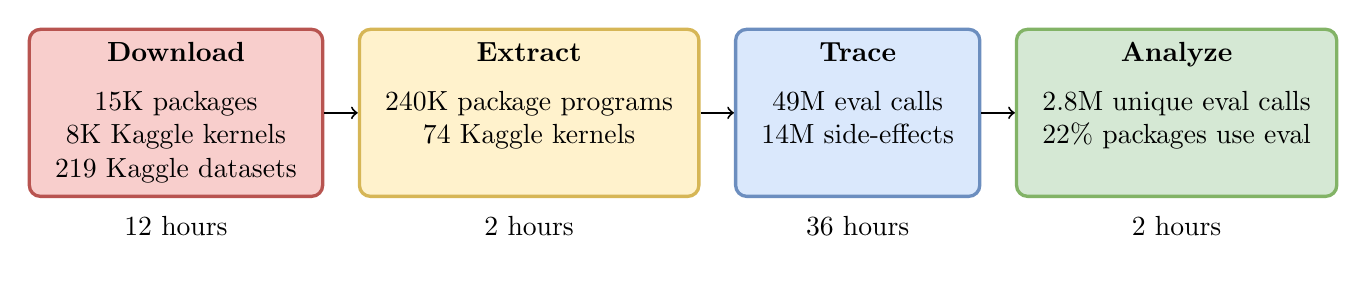
\begin{tikzpicture}
       \definecolor{red}{HTML}{F8CECC}
       \definecolor{darkred}{HTML}{B85450}
       \definecolor{yellow}{HTML}{FFF2CC}
       \definecolor{darkyellow}{HTML}{D6B656}
       \definecolor{blue}{HTML}{DAE8FC}
       \definecolor{darkblue}{HTML}{6C8EBF}
       \definecolor{green}{HTML}{D5E8D4}
       \definecolor{darkgreen}{HTML}{82B366}
       \newcommand{\nodesep}[0]{0.035 \textwidth}
       \newcommand{\textsep}[0]{0.005 \textwidth}
       \newcommand{\nodename}[1]{\begin{tabular}{c}#1\end{tabular}}
       \newcommand{\nodedesc}[1]{\begin{tabular}{c}#1\end{tabular}}
       \tikzstyle{block}     = [rectangle, rounded corners, minimum width=0.15 \textwidth, minimum height=60pt]
       \tikzstyle{connector} = [line width=0.25mm, ->]

       \node [block, fill = red, draw = darkred, very thick] (download) {
         \nodename{
           \vspace{1mm}\textbf{Download}\vspace{1mm}\\
           15K packages\\
           8K Kaggle kernels\\
           219 Kaggle datasets
         }
       };
       \node [below = \textsep of download]   (downloaddesc)   {\nodedesc{12 hours}};
       \node [block, right = \nodesep of download, fill = yellow, draw = darkyellow, very thick] (extract) {
         \nodename{
           \vspace{1mm}\textbf{Extract}\vspace{1mm}\\
           240K package programs\\%, 4.6M LOC\\
           74 Kaggle kernels\\%, 13K LOC\\
           \newline
         }
       };
       \node [below = \textsep of extract]   (extractdesc)   {\nodedesc{2 hours}};
       \node [block, right = \nodesep of extract, fill = blue, draw = darkblue, very thick] (trace) {
         \nodename{
           \vspace{1mm}\textbf{Trace}\vspace{1mm}\\
           49M eval calls \\
           14M side-effects\\
           \newline
         }
       };
       \node [below = \textsep of trace]     (tracedesc)     {\nodedesc{36 hours}};
       \node [block, right = \nodesep of trace, fill = green, draw = darkgreen, very thick] (analyze) {
         \nodename{
           \vspace{1mm}\textbf{Analyze}\vspace{1mm}\\
           2.8M unique eval calls\\
           22\% packages use eval\\
           \newline
         }
       };
       \node [below = \textsep of analyze]    (analyzedesc)    {\nodedesc{2 hours}};
       \draw [connector] (download)   edge (extract);
       \draw [connector] (extract)    edge (trace);
       \draw [connector] (trace)      edge (analyze);
     \end{tikzpicture}
   }
   \caption{Pipeline}\label{fig:pipeline}
 \end{figure}

\begin{compactenum}[(1)]
\item \emph{Download.} Packages are downloaded from CRAN, for Kaggle a web
  crawler retrieves code, and a command-line tool gets data. Installation is
  complicated by native dependencies which sometimes have to be resolved
  manually.
\item \emph{Extract.} The \genthat tool extracts all runnable code snippets and
  turns each of these into a self-standing program~\cite{issta18}, \c{knitr}
  extracts code from notebooks. Each extracted script is instrumented with calls
  to our dynamic analyzer in a way that avoid recording calls to \eval
  originating from our execution harness.
\item \emph{Trace.} Script run with a modified R interpreter to capture
  execution traces. Each script is run in its own process with the GNU R
  compiler turned off to avoid recording its execution. CRAN scripts run twice,
  once to capture \eval calls originating from package code and a second time to
  capture calls coming from base libraries.
\item \emph{Analyze.} Analysis outputs are merged, cleaned, and summarized.
  RMarkdown notebooks process the summarized data to generate all graphs (PDF
  from \c{ggplot2}) and numbers (exported as \LaTeX macros) appearing in the
  paper.
\end{compactenum}

 The pipeline runs in parallel~\cite{GNUparallel} orchestrated by a
Makefile. Servers have identical environments thanks to a docker image with all
dependencies installed.

\subsection{Dynamic Analysis}

The tracer that performs dynamic analysis of R scripts is built on top of
\rdyntrace, an extended R 4.0.2 virtual machine that exposes callbacks for
various runtime events~\cite{oopsla19b}. The tracer registers callbacks to all
variants of \eval and a few additional functions to locate the origin of \eval
arguments (it taints the results of calls to \c{parse} and \c{match.call}). It
captures dynamic code loading, as well as variable definition and assignment,
allowing us to record side effects that happen in environments while evaluating
code in \eval. A challenge was that lack of source code references for
expression that are not within block surrounded by braces. This is unfortunately
not easily fixed. We extend our dynamic analysis tool to attach synthetic source
code references to all \eval call sites, but the approach fails in some edge
cases. For performance reasons, the tracer is an R package written in C++ (3.2K
LOC) and R (1.3K LOC). While in theory the implementation should be
straightforward, not so in practice. Lazy evaluation requires delaying the
processing of arguments until (and if) they are forced. Accounting for
side-effects performed in an \eval is complicated by the fact that R is
implemented in a mixture of R and C, and that the language implementation can
call \eval. Lastly, large code bases exercise many edge cases of the highly
underspecified R behavior.

\paragraph{Limitations.} Even with the extension described above, there are
\PkgUndefinedRnd \eval calls without source information (\PkgUndefinedRatio of
all \eval calls). This happen when \eval is an argument to a higher-order
function or when it is called from native code. An other limitation is that we
do not record calls to the native \eval. Neither of these limitations should
invalidate our conclusions.

%%%%%%%%%%%%%%%%%%%%%%%%%%%%%%%%%%%%%%%%%%%%%%%%%%%%%%%%%%%%%%%%%%
\section{Measuring Eval}
%%%%%%%%%%%%%%%%%%%%%%%%%%%%%%%%%%%%%%%%%%%%%%%%%%%%%%%%%%%%%%%%%%

This section reports on the frequency of \eval in CRAN. We use \emph{site} to
refer to an occurrence of a call site to the \eval function in the source code
and \emph{call} to denote an observed invocation of the \eval function.

There are \PkgEvalCallSites \eval sites in \PkgPackages packages;
\PkgPackagesRatio packages use \eval. Over half of these packages have fewer
than 3 sites, and with the exception \MaxEvalCallSitesPackage which has
\MaxEvalCallSitesCount sites, all packages contain fewer than
\MaxEvalCallSitesRest sites. Fig~\ref{fig:pkgs-eval-callsites-hist} shows a
histogram of sites per package. Sites appear in \PkgFunsWithEval functions;
\CranFunsWithEvalRatio of all functions use \eval.


\begin{figure}[!b]
\centering
  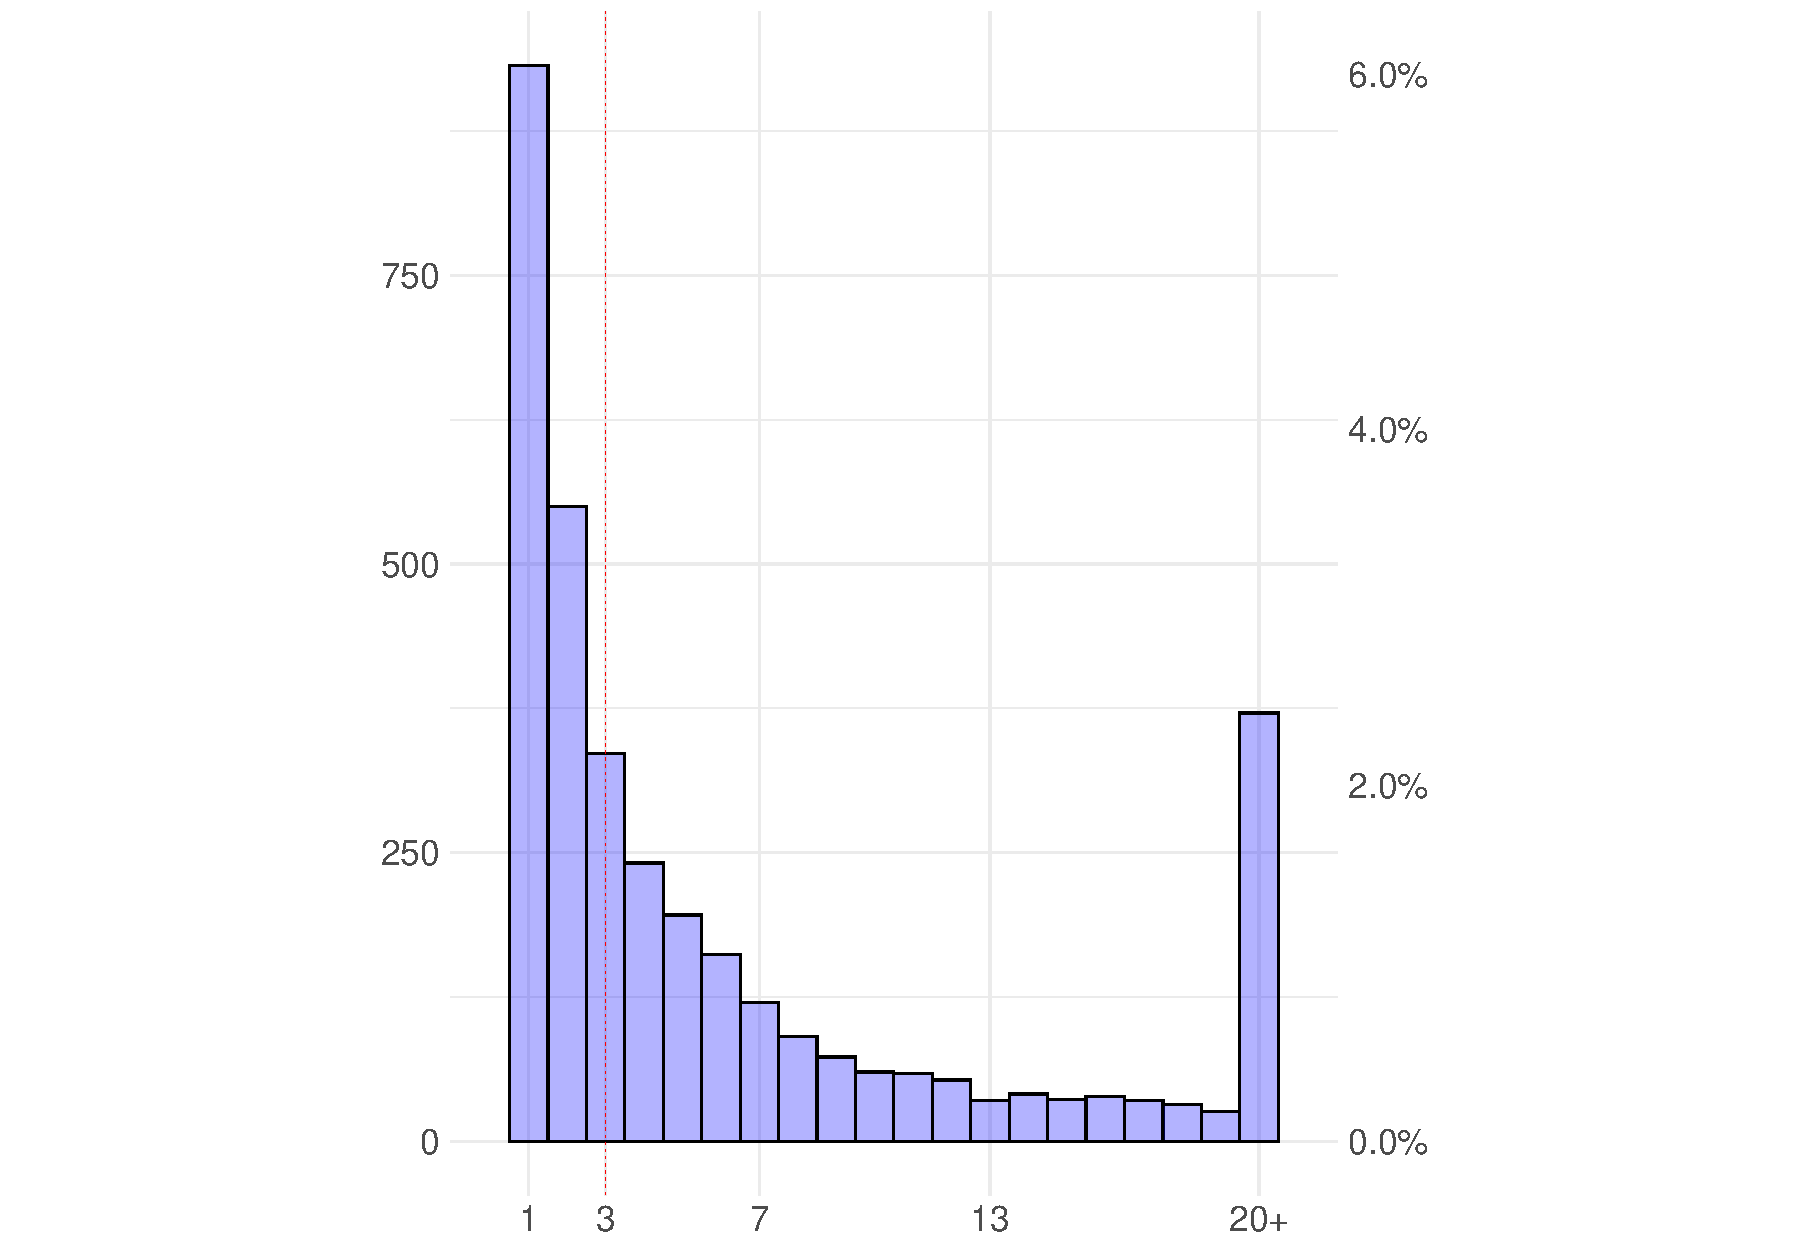
\includegraphics[width=10cm]{pkgs-eval-callsites-hist.pdf}
  \caption{ \eval call sites}\label{fig:pkgs-eval-callsites-hist}

\medskip
  \medskip

  \small
\begin{tabular}{@{}l@{\hspace{1.5cm}}l@{}}
\begin{minipage} {5cm}\small
  \begin{tabular}{r@{\,}r@{\,}l@{}r|r@{\,}r@{\,}l@{}r} \toprule
    \multicolumn{3}{c}{\bf \small\#calls} &\bf \small \#pck
&     \multicolumn{3}{c}{\bf \small\#calls} &\bf \small\#pck \\\midrule
\tt 1 &--& \tt 10      & \packageBina  & \tt 10K &--&\tt 100K  & \packageBine\\
\tt 11 &--& \tt 100    & \packageBinb  & \tt 100K &--&\tt 1M  & \packageBinf\\
\tt 101 &--& \tt 1K    & \packageBinc  & \tt 1M &--&\tt 10M   & \packageBing\\
\tt 1K &--& \tt 10K    & \packageBind  & \tt 10M &--& \tt 100M & \packageBinh\\\bottomrule
\end{tabular}
\caption{Call frequency}\label{freq}
\end{minipage}
&
\begin{minipage}{7cm}\small
\begin{tabular}{@{\,}r|rrrr}\toprule
  &\bf \eval & \bf \c{\bf evalq} & \c{\bf eval} & \c{\bf local}\\[-1.5mm]
           & & & \c{\bf .parent} &\\\midrule
\small Static sites &\packageStaticeval&\packageStaticevalq&\packageStaticevalparent&\packageStaticlocal \\
\small Exercised sites&\packageTriggeredeval&\packageTriggeredevalq&\packageTriggeredevalparent&\packageTriggeredlocal\\
\small Invocations&\packageEvalsRnd&\packageEvalqsRnd&\packageEparentsRnd&\packageLocalsRnd\\\bottomrule
\end{tabular}~\\[2mm]\caption{Variants}\label{tab:variantseval}
\end{minipage}\end{tabular}

\medskip

\includegraphics[width=.8\textwidth]{traced-eval-callsites.pdf} \centering
  \caption{\eval call sites coverage of the \PkgPackages packages.}%
  \label{fig:traced-eval-callsites}
\end{figure}


Our pipeline runs \CranRunnableScripts scripts extracted from \CranPackages
packages. Any run that does not call \eval is discarded, leaving us with
\packageNbruns runs. In these runs, \packageAllcalls \eval calls were recorded
originating from \PkgHitEvalCallSites sites. The runs exercised
\PkgHitEvalCallSitesAvgRatio of sites, a ratio similar to the package code
coverage metric which is \PkgCodeCoverage. The reasons some sites are not
exercised can be chalked down to incomplete tests and analysis failures
(\PkgFailedProgramsRatio of the runs crashed or timed out).
Fig.~\ref{fig:traced-eval-callsites} plots exercised site with respect to all
sites for each program; as can be seen coverage is unequal.
Fig.~\ref{freq} summarizes the frequency of calls, call counts on the left and
number of packages on the right. There are \packageFewcalls packages with fewer
than 100 calls, and \packageManycalls packages with more than 1,000 calls.
\packageMaxcallspack calls \eval \packageMaxcalls times and thus accounts for
over half of our observations.
Fig.~\ref{tab:variantseval} summarizes use of variants, the first row has sites
(\emph{static}), the second has sites encountered during analysis
(\emph{exercised}) and the last gives calls (\emph{invocations}). Most sites and
calls go to \eval itself, \c{eval.parent} is rare, and both \c{evalq} and
\c{local} are barely used at all.

\begin{wrapfigure}{r}{5cm}  \small  \vspace*{-2mm}\centering
  \begin{tabular}{r@{\,}r@{\,}l@{\,}r|r@{\,}r@{\,}l@{}r} \toprule
    \multicolumn{3}{c}{\bf \#calls} & \bf \#sites &
     \multicolumn{3}{c}{\bf \#calls} & \bf \#sites \\\midrule
    \tt 0 &--& \tt 50    & \packageRunbina & \tt 501 &--& \tt 1000   & \packageRunbine\\
    \tt 51 &--& \tt 100  & \packageRunbinb & \tt 1001 &--& \tt 1500  & \packageRunbinf\\
    \tt 101 &--& \tt 250 & \packageRunbinc & \tt 1501 &--& \tt 2000  & \packageRunbing\\
    \tt 251 &--& \tt 500 & \packageRunbind & \tt 2001 &--& \tt 3000 & \packageRunbinh\\\bottomrule
  \end{tabular}
  \caption{Normalized calls} \label{cn}
\end{wrapfigure}

Fig.~\ref{cn} shows average count of calls from a given site and given run and
how many sites fall in that range. For instance, \packageRunbinh sites are
called over 2,000 times per run. Larger call counts suggest the presence of
loops or recursive functions, but given the data this seems to be the exception;
\packageRunbina of sites are called fewer than 50 times, most sites are invoked
once and half as many are invoked twice.

\Eval accepts any value as argument, but if the value is not an expression,
\eval returns it unchanged. Expressions account for \packageCodepercent of
arguments. More specifically, \packageSymbolpercent are \c{symbol}s (variables
such as \c{x}), \packageLanguagepercent are \c{language} objects (expressions
representing a function calls), and \packageExpressionpercent are \c{expression}
objects (lists of expressions). Further inspection reveals that \c{\_inherit}
accounts for \packageGgplotsymbolpercent of symbols and comes from one site in
\c{ggplot2}.\footnote{Each object has a field model inheritance, this comes from
\c{ggproto}, one of the many object-oriented systems for R.}


\begin{wrapfigure}{r}{6.2cm}
\begin{tabular}{c}
{\hspace{-25mm}\includegraphics[width=0.8\textwidth]{package_size_loaded_distribution}}
\end{tabular}
\caption{Loaded code} \label{fig:sizedistribution}
\end{wrapfigure}

To estimate how much executable code is injected through \eval, we measure the
size of the arguments in terms of number of nodes. For example,
\c{expression(x+1)} has a size of 3. The large number of symbols skew the median
to \packageMedianszeval but the average size is \packageAvgszeval nodes. The
largest \eval input we observed was an expression of \packageMaxszeval nodes, a
significant chunk of code. Fig.~\ref{fig:sizedistribution} shows the
distribution of sizes for arguments of fewer than 25 nodes. Sizes drop rapidly,
there are few observations larger than 15 nodes. The long tail is omitted for
legibility. As an alternative to counting nodes, we tried measuring string
lengths of expressions after calling a function to deparse values back to
strings, but these measurements were dominated by massive data objects which
could range in the MBs.

To assess how much computational work is performed in \evals, we count the
instructions executed by the interpreter. Most call do relatively little, with
\packageSmalleventspct of calls executing fewer than 50 instructions. The violin
plot of Fig.~\ref{ev}(a) shows the distribution of short running \evals; the
data is dominated by \evals which simply perform symbol lookup. Fig.~\ref{ev}(b)
shows the distribution of work-intensive \evals which go all the way to
\packageMaxeventsRnd instructions.

\begin{figure}[h!]
\begin{tabular}{@{}c@{}c@{}}
\begin{minipage}{7.5cm}
 \includegraphics[width=\textwidth]{package_events_per_pack_small}
\end{minipage}&\begin{minipage}{7.5cm}
  \includegraphics[width=\textwidth]{package_events_per_pack_large}
\end{minipage}\\[-3mm]
\small (a) Small & \small (b) Large
\end{tabular}
 \caption{Instructions per call} \label{ev}
\end{figure}

\paragraph{Discussion.}
\Eval is widely used in CRAN packages. Nearly every fourth package contains at
least one \eval call site. However, most packages use \eval modestly. Packages
that rely heavily on \eval are mostly ones that provide statistical modeling and
simulation functions. At runtime, over a third of our scripts triggered calls to
\eval, note that all scripts performed \eval originating from base package but
these are disregarded here. Half of the calls come from a single site, for the
rest, most packages have low call frequency. The data is consistent with usage
of \eval for configuration and meta-programming and not in performance sensitive
contexts such as loops. While most arguments to \eval are small, often just a
variable name, and do little work, we have also observed large \eval arguments
and arguments that perform massive amounts of work.

%%%%%%%%%%%%%%%%%%%%%%%%%%%%%%%%%%%%%%%%%%%%%%%%%%%%%%%%%%%%%%%%%%%%%%%%%
%%%%%%%%%%%%%%%%%%%%%%%%%%%%%%%%%%%%%%%%%%%%%%%%%%%%%%%%%%%%%%%%%%%%%%%%%
\section{A Taxonomy of \Eval}

The previous section gave a quantitative view of \eval usage; we now try to
elucidate \emph{what} it does.

\subsection{The expression in \eval} \label{sec:minimized}

\begin{table}[!b]\small
\begin{tabular}{crrrrrc}\toprule
  \bf $min(e)$& \bf \#sites & \bf \%sites & \bf \#packages & \bf \#operations & \bf \%envir & \bf example\\\midrule
\c X&\packageMinimizedcallsitesa &\packageMinimizedpropsitesa &\packageMinimizedpackagea &\packageMinimizedmedianoperationsaRnd &\packageMinimizedpercentparentframesa & \c{y+1}\\
\c{F(F(X))} & \packageMinimizedcallsitesb  & \packageMinimizedpropsitesb & \packageMinimizedpackageb  & \packageMinimizedmedianoperationsbRnd & \packageMinimizedpercentparentframesb & \c{gbov( mean(x), a-1)}\\
\c{V}&\packageMinimizedcallsitesc &\packageMinimizedpropsitesc &\packageMinimizedpackagec &\packageMinimizedmedianoperationscRnd &\packageMinimizedpercentparentframesc& \c{c(42,21,0)}\\
\c{F(X)}& \packageMinimizedcallsitesd & \packageMinimizedpropsitesd & \packageMinimizedpackaged & \packageMinimizedmedianoperationsdRnd & \packageMinimizedpercentparentframesd & \c{seq\_len(iters)} \\
\c{\$} & \packageMinimizedcallsitese & \packageMinimizedpropsitese & \packageMinimizedpackagee & \packageMinimizedmedianoperationseRnd & \packageMinimizedpercentparentframese & \c{DF\$B}\\
\c{model.frame}& \packageMinimizedcallsitesf & \packageMinimizedpropsitesf & \packageMinimizedpackagef & \packageMinimizedmedianoperationsfRnd & \packageMinimizedpercentparentframesf &  \c{model.frame(formula = Z $\sim$ U)}   \\
\c{F()}& \packageMinimizedcallsitesg & \packageMinimizedpropsitesg & \packageMinimizedpackageg & \packageMinimizedmedianoperationsgRnd & \packageMinimizedpercentparentframesg & \c{rgamma(3, 2, n = 10L)} \\
\c{FUN} & \packageMinimizedcallsitesh & \packageMinimizedpropsitesh & \packageMinimizedpackageh & \packageMinimizedmedianoperationshRnd & \packageMinimizedpercentparentframesh & \c{function(x, y) x + 3 * y} \\
\c{<-} & \packageMinimizedcallsitesi  & \packageMinimizedpropsitesi & \packageMinimizedpackagei & \packageMinimizedmedianoperationsiRnd & \packageMinimizedpercentparentframesi & \c{x[1, 2:3, 2:3] <- value}\\
\c{BLOCK} & \packageMinimizedcallsitesj & \packageMinimizedpropsitesj & \packageMinimizedpackagej & \packageMinimizedmedianoperationsjRnd & \packageMinimizedpercentparentframesj & \c{\{ write.csv(iris, tf) ; file.size(tf) \}} \\\bottomrule
\end{tabular}
\caption{Minimized expressions} \label{tab:minimizedexpressions}
\end{table}


The expressions passed to \eval vary widely. We categorize expressions using a
minimization function which abstract some of the incidental details of
expressions and return a ``shape'' that can be used to group similar \evals. The
function $min(e)$ which for a given expression $e$ returns a normal form. Normal
forms use \c V to stand in for values occurring in expression, \c X stands in
for variables, and \c F stands for functions. The function performs constant
folding of arithmetic and string expressions over base operators, for instance
$min(\c{1+1})$ simplifies to $\c{V}$, on the ground that addition of values
likely returns a value. Value simplification takes $min(\c{c(1,2,3+2)})$ to
$\c{V}$ as a complex vector containing values is a value. Variable absorption
has $min(\c{x+y})$ becomes $\c{X}$, this motivated by the fact that addition is
not an ``interesting'' operation, and that \c X stands in for any number of
variable lookups. Function absorption simplifies nested functions to keep an
abstraction of the nesting $min(\c{g(f(x),h(z))})=\c{F(F(X))}$. There are other
simplifications, the full list can be found in our artifact. It is worth
mentioning that these simplifications are heuristics, in R \c{1+1} is not
necessary \c 2. The addition operator can be redefined, but it typically isn't
or at least not in a way that would invalidate arithmetic.

Table~\ref{tab:minimizedexpressions} gives the 10 most frequent shapes with the
number and ratio of sites that received arguments of that shape. Operations is
the median count of instructions performed by the interpreter when evaluating
argument of the given shape. Envir is the ratio of sites that evaluate in a
function environment. The last column has a sample expression that normalizes to
the corresponding shape. We detail these shapes and discuss their implication for
the behavior of \eval.

\newcommand{\EE}[1]{{{\emph{\framebox{#1}}}}\\[1mm]}

\begin{tabular}{@{}p{.97\linewidth}}
  \medskip\EE{$min(e)=\c{V}$} \\[-2mm]\small Values occur in 16\% of sites, 74\% of
  those are constants such as integers, the remainder evaluate to a value. \Eval
  is needed when the expression denoting the values is constructed
  programmatically. Cases when a value is directly given to \eval, and \eval
  returns it unchanged, often occur when a computation has a default path and
  another, more interesting, path that requires evaluation. The following is a
  call site that always see a string; \packageNbCallSitesUniqueActualValue of
  sites only ever see a value. This shape usually run in few interpreter steps.
  The environment in which they evaluate is mostly irrelevant.
\begin{lstlisting}
  eval(paste("A~",paste(paste(names(X[,-1])),collapse="+")))
\end{lstlisting}
\\
\medskip\EE{$min(e)=\c{X}$}\\[-2mm]\small Variable lookups are the most common shape,
\packageNbSymbolVarSitePercent are simple variable names, e.g. \c x. The shapes
subsumes \c{V} and built-in arithmetic operations, so a mixture of arithmetics
and variables normalize to \c X. A lookup is one step of execution, if a promise
is returned an arbitrary number of additional steps may be needed; the median is
\packageMinimizedmedianoperationsaRnd, suggesting that most variable read do
little work. Variables are often evaluated in environments that have been
constructed programmatically, \packageMinimizedpercentparentframesa of
expressions are evaluated in a function environment.
\\
\medskip\EE{$min(e)=\c{\$}$}\\[-2mm]\small This shape extends \c X to include lookup
with the dollar operator, \eg~\c{x\$f}, and vector indexing, \eg~\c{x[42]} and
\c{x[[24]]}. This takes a few more step of evaluation on average, and is
typically used in a function environment.
\\
\medskip\EE{$min(e)=$~\c{<-}}\\[-2mm]\small This includes both direct assignment {\tt
  <-} and parent environment assignment {\tt <\,\!<-} as well as the \c{assign}
function. It subsumes \c{\$}. Assignments
represent the most obvious source of side effects in \eval.
\\
\medskip\EE{$min(e)=\c{F()}$}\\[-2mm]\small Function calls without variable lookups or
assignment. A variable is allowed the function position, looking up
functions does not trigger computation unless the function's name
is bound to a promise. This shape typically does not perform much work.
\\
\medskip\framebox{$min(e)=\c{F(X)}$}~\EE{$min(e)=\c{F(F(X))}$}\\[-2mm]\small Function
calls whose arguments may include variable references and nested calls. Together
they represent the most frequent shape and perform over 16 steps. They are
frequently evaluated in function environments.
\end{tabular}

\begin{tabular}{@{}p{.97\linewidth}}
  \medskip\EE{$min(e)=\c{FUN}$}\\[-2mm]\small Function definitions without any
  computation, \eg~\c{function(x) x+1}. In addition to \c{FUN},
  \packageGeneralizedFunctionDefinitionSitesPercent of sites have function
  definitions nested in other expressions.
\\
\medskip\EE{$min(e)=\c{BLOCK}$}\\[-2mm]\small Multi-statement code blocks, as
they can be large we do not try to normalize their contents. They execute in a
median \packageMinimizedmedianoperationsjRnd steps, usually, in function
environments.
\\
\medskip\EE{$min(e)=\c{model.frame}$}\\[-2mm]\small The \c{model.frame} function
returns a dataframe resulting from fitting the model described in a formula.
This shape subsumes \c{F(F(X))}, \c{FUN}, and assignments. It is the single most
popular function invoked from \eval. Each call does a median of 2K instructions.
\end{tabular}

\paragraph{Discussion.} The number of different shapes that any given
\eval site sees is an indication of the versatility of that site.
\packageNbOneMinimizedPercent of sites only see a single expression shape. It
would be encouraging if one could, given a small training set, predict the shape
of \evals to come. In our corpus, only a few sites are highly polymorphic with
more than eight shapes. An example of those is the pipe operator of the
\c{magrittr} package which is used to compose functions, \eg instead of
\c{f(g(h(x),y),z)} one can write \c{h(x) \%>\% g(y) \%>\% f(z)}. As there many
different patterns of use, there are also many different shapes. In comparison
with R, JavaScript's \eval usage was more straightforward and more predictable
as reported by \citet{oopsla12b}, with 98\% of sites with only one shape. On the
other hand, there are \packageNbSimpleMinimizedOne sites that only receive one
of the simple shape (\ie\xspace \c{X}, \c{V}, \c{\$} or \c{<-}), and
\packageNbSimpleMinimizedMore sites get multiple simple shapes. Among these
sites, there are many cases where \eval could be replaced by simpler constructs
such as \c{get} to lookup a name in an environment, \c{assign} to set a value to
a name in an environment, or \c{do.call} to call a function reflectively.

\subsection{The environments of \eval}\label{sec:env}

Contrary to JavaScript, in R the environment of \eval can be specifies by its
\c{env} argument. This gives users control over what is visible to the
computation started by \eval and the potential reach of its side-effects. We
distinguish the following kinds of environments:

\begin{itemize}[---]
\item \emph{Function:} environments for the local variables of some function
  currently active on the call stack. Obtained by calling \c{parent.frame()} or
  \c{sys.frame()}.
\item \emph{Synthetic:} environments built from data structures such as lists,
  data.frames, or constructed explicitly with \c{new.env}, \c{list2env}, or
  \c{as.environment} or the empty environment.
\item \emph{Global:} environments in which scripts or interactive commands are
  evaluated.
\item \emph{Package:} environments of libraries.
\end{itemize}


Table~\ref{tab:highlevelenvironments} shows that most calls evaluate in the
scope of a function, global is a distant second. This means that most reads and
writes act on local variables. But of which function? Table~\ref{tab:funoffset}
gives the offset of that function on the call stack: 0 is function that called
\eval, 1 is that function's caller, and so on. In 81\% of cases, \eval is
resolved the caller -- the variables of the function where the call to \eval
textually occurs are read and written. About 1.5\% of sites evaluate their
argument three frames up the call stack, or above. Modular reasoning is thus
impossible in R. Since the actions of \eval happen at a distance, understanding
any given code snippet requires knowing which functions may be called
transitively from that snippet. In \packageNbOneCategoryEnvirSitePercent of
sites, only kind of environment is observed.

\begin{table}[h]
  \centering\small\hspace{-.5cm}
\begin{minipage}{3.7cm}
  \begin{tabular}{@{}rrr@{}}\toprule
 \bf Kind & \bf \#sites & \bf \%sites \\\midrule
 Function & \packageNbFunctionEnvSites &  \packageNbFunctionEnvSitePercent\\
 Synthetic & \packageNbSyntheticEnvSites & \packageNbSyntheticEnvSitePercent \\
 Global &  \packageNbStrictGlobalEnvSites & \packageNbStrictGlobalEnvSitePercent \\
 Package & \packageNbPackageNamespaceEnvSites & \packageNbPackageNamespaceEnvSitePercent \\\bottomrule
\end{tabular}
\caption{Kinds per site} \label{tab:highlevelenvironments}
\end{minipage}\hspace{-.2cm}
\begin{minipage}{3.7cm}\centering
  \begin{tabular}{@{}rrr@{}}\toprule
 \bf Offset & \bf \#sites & \bf \%sites \\\midrule
  \packageCallerEnvHierarchyNamea & \packageCallerEnvHierarchySitesaRnd & \packageCallerEnvHierarchySitePercenta \\
  \packageCallerEnvHierarchyNameb& \packageCallerEnvHierarchySitesbRnd & \packageCallerEnvHierarchySitePercentb \\
  \packageCallerEnvHierarchyNamec& \packageCallerEnvHierarchySitescRnd & \packageCallerEnvHierarchySitePercentc  \\
$\ge 3$& \packageNbFarAwayCallerSites &  \packageNbFarAwayCallerSitePercent \\\bottomrule
 \end{tabular}
\caption{Function offset}\label{tab:funoffset}
\end{minipage}\hspace{-.2cm}
\begin{minipage}{3.7cm}
  \begin{tabular}{@{}rrr@{}} \toprule
\bf Parent & \bf \#sites & \bf \%sites \\\midrule
Function & \packageNewEnvCategorySitesa & \packageNewEnvCategorySitePercenta \\
Package & \packageNewEnvCategorySitesb &  \packageNewEnvCategorySitePercentb\\
Global & \packageNewEnvCategorySitesc & \packageNewEnvCategorySitePercentc \\
    Empty & \packageNewEnvCategorySitesd & \packageNewEnvCategorySitePercentd \\\bottomrule
\end{tabular}
\caption{Wrapper envs.} \label{tab:newenvs}
\end{minipage}\hspace{-.2cm}
\begin{minipage}{3.7cm}\centering
  \begin{tabular}{@{}ccc@{}} \toprule
 \bf \#kinds & \bf \#sites &  \bf \%sites \\\midrule
 \packageNbCategoryEnvira & \packageNbCategoryEnvirSitesaRnd &  \packageNbCategoryEnvirPercenta\\
 \packageNbCategoryEnvirb &  \packageNbCategoryEnvirSitesbRnd & \packageNbCategoryEnvirPercentb \\
 \packageNbCategoryEnvirc & \packageNbCategoryEnvirSitescRnd &  \packageNbCategoryEnvirPercentc\\
 \packageNbCategoryEnvird & \packageNbCategoryEnvirSitesdRnd & \packageNbCategoryEnvirPercentd\\\bottomrule
\end{tabular}\caption{Multiplicities}\label{tab:polyenvir}
\end{minipage}\hspace{-1cm}
\end{table}

Each synthetic environment has parent that is specified when calling
\c{new.env}. When \c{envir} is a list or a data frame, \eval uses its third
argument (\c{enclos}). The parent is used to search for variables not found in
its child (side-effects stay in the child). Table~\ref{tab:newenvs} shows parent
kinds for synthetic environments. Most of them are functions.

Global \evals split between intentional and accidental one. Direct references to
the top-level, using \c{globalenv()} or \c{.GlobalEnv}, are rare; they occur in
only \packageNbExplicitGlobalSites sites. Thus we suspect most uses of global
are accidental. They arise from the fact that our corpus, consists of many code
snippet that are run at top-level, global is thus the caller of \eval. This
noteworthy because writes to global variables are visible to all functions and
are not reclaimed by the garbage collector. So accidental uses may pollute that
namespace. Table~\ref{tab:polyenvir} gives the number of kinds seen at a given
call site.

\paragraph{Discussion.}
The data presented here is not surprising. The main use of \eval is to provide a
customizable extension mechanism for the behavior of functions. They are a way
to parameterize the function with any behavior that can be expressed in R. The
behavior of \eval within its enclosing function is to read and write variables,
mostly read, and very rarely delete variables. There are also some cases where
new variables are injected in a function. Usually, this in the direct caller,
but can sometimes take effect several frames up the call stack. There is
something brittle about code relying on the position of a caller, many
refactorings may break code that does that.

One bit of information that we lack is how the environment was obtained. Our
expectation is that the expression was extracted from a promise using
\c{substitute}, perhaps modified, and then evaluated with the environment coming
from the same promise. We believe the case where \eval is provided the results
of programmatically selecting some call stack to be less frequent.

Synthetic environments are relatively frequent. Common uses-case include
evaluation of an expression in a sandbox, or using a data structure as
environment, for example one could evaluate a method of an object and use and
environment to hold the object's fields.

We have already explained the popularity of global environments, as for package
environments, they are used in only \packageNbPackageNamespaceEnvSites sites.
This is probably for the best as mutating the bindings of a loaded package is
frowned upon and R tries to discourage it.

\subsection{The origins of \eval}

Where does the expression passed to \eval come from? There are various means of
creating an expression, often these means correlate with a particular use case.
Our analysis records the values returned by some functions of interest as well
as their arguments. We build a direct acyclic graph that track the provenance of
the values that are given to \eval. The following example yields the provenance
graph with five nodes on Figure~\ref{fig:provgraph} for expression \c{e}.

\begin{lstlisting}
 > e <- parse(text = "a ; b")
 > e[[2]] <- quote(c)
 > eval(e)
\end{lstlisting}

\begin{figure}[h]\centering
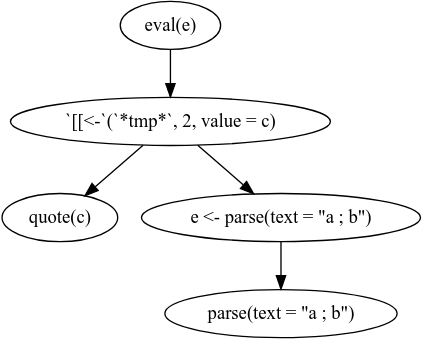
\includegraphics[width=5cm]{provenance-graph}
\caption{Provenance} \label{fig:provgraph}
\end{figure}

The provenance of \c{e} includes both \c{parse} and \c{quote}. We pick an origin
by traversing the graph from the root, following the left-hand side member of
assignments until a leaf. It represents the provenance that is further modified
to yield the expression passed to \eval. In our example, the origin is \c{parse}.

% Wrap tables do not play well with lists (they warn about it in the documentation actually!)
\begin{wraptable}{r}{5cm}\small\centering
\begin{tabular}{lcc}\toprule
\bf Provenance & \bf \#sites & \bf \%sites \\\midrule
		\packageProvenanceNamea & \packageNbProvenanceSitesa & \packagePercentProvenanceSitesa \\
		\packageProvenanceNameb & \packageNbProvenanceSitesb & \packagePercentProvenanceSitesb \\
		\packageProvenanceNamec & \packageNbProvenanceSitesc & \packagePercentProvenanceSitesc \\
		\packageProvenanceNamee & \packageNbProvenanceSitese & \packagePercentProvenanceSitese \\
		\packageProvenanceNamef & \packageNbProvenanceSitesf & \packagePercentProvenanceSitesf \\
		\packageProvenanceNameg & \packageNbProvenanceSitesg & \packagePercentProvenanceSitesg \\
		\packageProvenanceNameh & \packageNbProvenanceSitesh & \packagePercentProvenanceSitesh \\
		\packageProvenanceNamei & \packageNbProvenanceSitesi & \packagePercentProvenanceSitesi \\
		\packageProvenanceNamel & \packageNbProvenanceSitesl & \packagePercentProvenanceSitesl \\
		\packageProvenanceNamen & \packageNbProvenanceSitesn & \packagePercentProvenanceSitesn \\\bottomrule
\end{tabular}
\caption{Origin} \label{tab:detailed_provenances}
\medskip
\begin{tabular}{rrr} \toprule
\bf Origin  & \bf \#sites & \bf \%sites \\\midrule
Reflection &  \packageNbReflectionSites & \packageReflectionSitesPercent\\
String & \packageNbStringSites & \packageStringSitesPercent \\
Constructed & \packageNbConstructedSites & \packageConstructedSitesPercent \\
Environment & \packageNbSymbolSites & \packageSymbolSitesPercent \\
External & \packageNbExternalSites & \packageExternalSitesPercent \\\bottomrule
\end{tabular}
\caption{Provenance}\label{tab:provenance}
\end{wraptable}

Table~\ref{tab:detailed_provenances} shows frequencies of provenance. For
technical reasons, we misclassify a small number of sites. Manual inspection of
numerous examples suggests that errors are rare. We further classify them into
high-level categories:

\begin{itemize}[---]
\item {\it Reflection:} use of \c{match.call} to reflectively capture the
  expression that invoked this function, arguments are promises, and
  \c{substitute} is used to retrieve their source.
\item {\it String:} create from strings by invoking \c{parse},
  \c{str2expression}, or \c{str2lang}.
\item {\it Constructed:} invoked \c{quote} or \c{expression}, or by built with
  \c{call} or \c{as.call}.
\item {\it Environment: } created with \c{as.name} or \c{as.symbol}, typically
  to read a non-local environment.
\item {\it External: }  call to a C function. % Put an example
\end{itemize}

Table~\ref{tab:provenance} summarizes provenance. Some sites are invoked with
different provenances, they are counted multiple times. Strings correlate with
dynamic code loading as done by \c{source} and \c{sys.source}. Few calls
(\packageNbParseFromFileSites in total) consume the result of calling \c{parse}
on a file. Most build strings programmatically. We identified one function
\c{invokeRestartInteractively} that prompts the user for input and \evals it.




\paragraph{Discussion}
The main use case for \eval involves using \c{match.call}, \c{substitute}, or
\c{match.call} to access and transform arguments of a function. Constructing
expressions from strings is also a common use case. The constructed category
shows that most \evals comes from existing code that was modified by the
programmer before invoking \eval. Both constructed and reflection categories
roughly correspond to meta-programming. Some use cases could likely be replaced
by macros if the R designers could be convinced to overcome their distaste for
those. Another use of \eval is to directly build symbols to evaluate them in
another environment.

\subsection{The effects of \eval}

\Eval may perform side-effects. We care about effects that are visible after a
call finishes, \ie variable definitions, updates, and removals. Knowing in which
environments these side-effects happen, can help determine the impact of \eval
on our ability to reason about the code. Our analysis records information about
every environment. From the recorded data, we discard side-effects coming from
unit testing frameworks as they use \eval to run all their tests and thus
dominate the side-effect data.\footnote{The corpus has \c{RUnit, testthat,
  tinytest} and \c{unitizer} testing frameworks.}

We record \SEAllRnd side-effects from \SEAllCallsRnd calls and \SEAllSites
sites. The challenge is to remove accidental side-effects caused by the R
virtual machine implementation and not user code. For example, the
\c{.Random.seed} variable is saved and restored from and to the global
environment every time a statistical routine is called. Filtering accidental
side-effects leaves us with \SEUserRnd writes from \SEUserCallsRnd calls (in
\SEUserSites sites and \SEUserFunctions functions). \SEFunsNighty functions are
responsible for 90\% of side effects. Half of those come from just three
functions: \c{plyr::allocate\_column} (allocates space for a new data frame
column), \c{withr::execute\_handlers} (executes deferred expressions), and
\c{foreach::doSEQ} (executes an expression on each element in a collection,
possibly in parallel). Most of the sites (\SESitesInEnvirRatio) update
the environment specified by the \c{env} parameter.

\begin{wraptable}{r}{7cm}\small\centering
  \begin{tabular}{lrrrr}
    \toprule
    \bf Environments & \bf \#sites & \bf \%sites & \bf \#funs. & \bf \%funs. \\%
    \midrule
    \expandableinput tag/table-se-target-envs.tex
    \bottomrule
  \end{tabular}
  \caption{Target environments for side-effects} \label{tab:se-env}
\end{wraptable}

Table~\ref{tab:se-env} shows environment kinds where side-effects happen.
Function environments distinguish between \emph{local}, the caller environment
(offset 0), and \emph{function} (offset >0). \emph{Synthetic} represents
constructed environments. \emph{Object} is used to denote the environments
attached to objects and classes in the S4 and R6 object systems. \emph{Multiple}
denotes cases where side-effects to more than one kind originate from one site.
The table gives the number of call sites of \eval (and the ratio) performing
side-effect in a particular environment kind. The table also gives the number of
functions in which these sites occur (and ratio).

Most sites, \SESitesInOneClass, do all their side-effects consistently in one
kind of environments. The same happens at the function level. Almost half of the
sites (over a third of the functions) do side effects in either \emph{Local} or
\emph{Object} environments. This gives a ray of hope for a hypothetical R
compiler. Even though \eval can do anything anywhere, the data suggests most
effects are sane.

Table~\ref{tab:se-types} shows recorded effects. There are over 5M updates. In
terms of calls, we see assignments primarily and in terms of site definitions.
This is expected. A subsequent \eval call will turn a definition into an update.
The most dangerous side effect is variable removal, as it means that after a
call to \eval some binding in some environments will disappear. While rare, this
happens, but the vast majority comes from a single site
(\c{withr::execute\_handlers}). This makes sense as it is used to defer
evaluation of an expression to after the function exit and thus used for clean
up. It is used almost exclusively by the \c{tidyselect} package for removing the
reference to the current quosure environment while interpreting a data frame
column selectors.\footnote{\cf \url{https://tidyselect.r-lib.org/}}

Looking closely at the value types in variable updates, we observe that the
majority of \eval sites involve basic R vectors (\SEBasicTypeRatio) and lists
(\SEListTypeRatio). From the compiler perspective, we would like to know how
many sites change function bindings. In the corpus, this happens in only
\SEClosureType sites; \SEClosureTypeLocal of them do that in the local
environment. We have manually inspected a few of these sites, but except for
manual injection of parameters into a \c{model.frame} execution environment, we
did not find a common use case.

\begin{table}[h]
  \small
  \centering
  \begin{tabular}{lrrrrrr}
    \toprule
    \bf Side effect & \bf \#events & \bf \%events & \bf \#calls & \bf \%calls & \bf \#sites & \bf \%sites \\%
    Side effect & \#events & \%events & \#calls & \%calls & \#sites & \%sites \\%
    \midrule
    \expandableinput tag/table-se-types.tex
    \bottomrule
  \end{tabular}
  \caption{Types of \eval side-effects} \label{tab:se-types}
\end{table}

Out of the minimized expressions, it is \c{BLOCK}, \c{<-} and
\c{F(F(X)} that contribute to the vast majority of side effects. Concretely,
92\% of \c{BLOCK}, 87\% of \c{<-} and 15\% of \c{F(F(X))} expressions contain
side effects. In the case of \c{BLOCK}, most of the side effects happen in the
environment passed to \eval (which by default is the parent environment, \ie
the local or function in our classification). For \c{<-} it is 15\%, however,
that is only because of the \c{plyr::allocate\_column} which does the side
effect in the environment containing the data frame that is the target for the
newly allocated column. Without this call, \c{<-} is similarly predictable with
96\% of side effects in the passed environment. For \c{F(F(X))} minimization
for, it is less clear as 48\% of side effects happen in a different environment
to the one that was passed to \eval.

\paragraph{Discussion} In JavaScript assignments in \eval can happen in either
local scope or less often, when called through an alias, in the global scope. In
R, given the support for first-class environments, it can happen anywhere,
making it \eval more dangerous than it already is. However, the data suggest
that first, side-effects from \eval are not as widespread as in the case of
JavaScript,\footnote{\citep{ecoop11} shows that in the \emph{Interactive}
scenario, \eval in Javascript performs, store events can reach up to 40\% of the
events, and 7\% to 8\% of the \eval do side effects in the global scope. } and
that over half of them happen in a predictable environment.

\section{Usage of \eval}

The R language was intended to be extensible. The combination of lazy
evaluation, \c{substitute} and \c{eval} are some of the tools given to
developers to this end. To understand \emph{why} developers use \eval, we
manually inspected top 117 \eval call-sites which contribute to 90\% of the
\eval calls. In this section, we give examples of the \eval usage from this
real-world sample. The examples are often simplified to fit the space and
increase clarity. For each example, we indicate the package and the function
where it is located.

\paragraph{Simplify Interfaces} A common use of \eval is to simplify interfaces by
letting users pass string argument which can be parsed and evaluated in custom a
environment. An example is the \code{rARS} function shown below. This function
is defined in the \code{AdapSamp} package that implements sampling algorithms.

\begin{figure}[h]
\begin{lstlisting}
rARS <- function(n, formula, min=-Inf, max=Inf, sp) {
    ...
    p <- function(x) { eval(parse(text=formula)) }
    ...
}
\end{lstlisting}
  \caption{AdapSamp::rARS}
\end{figure}

The \code{rARS} function take a \code{formula} argument, an expression in
\code{x} as a string, that represents the kernel of the target distribution.
This is turned into the closure \code{function(x) \{ eval(parse(text=formula))
  \}}. An alternative design would be to supply the closure itself as the
argument, but passing \code{function(x) exp(-x^2/2)} is probably not as
convenient for domain-experts as passing \code{"exp(-x^2/2)"}.

\paragraph{Code Generation} The \c{Rcpp} package which bridges R with C++ is a
popular user of this pattern. Its \code{.makeCppMethods} function, shown below,
uses \eval to automatically generate R bindings to native code. The expression
\code{function(...) .CppObject$WHAT(...), list(WHAT = as.name(what))} is
evaluated with different values of \code{what} to generate wrapper functions
which are assigned to the \code{methods} structure keyed by \code{what}.

\begin{figure}[h]
\begin{lstlisting}
.makeCppMethods <- function(methods, cppclassinfo, env) {
    ...
    for(what in cppMethods[! cppMethods %in% newMethods])
        methods[[what]] <- eval(substitute(
                  function(...) .CppObject$WHAT(...), list(WHAT = as.name(what))), env)
    ...
}
\end{lstlisting}
  \caption{Rcpp::.makeCppMethods}
\end{figure}

\paragraph{Extracting varargs} A surprising use of \eval is the
extraction of unevaluated text of arguments passed to a \code{...} parameter.
Consider the definition of the \code{NVL} function from the
\code{statnet.common} package. This function returns the first argument that is
non \code{NULL}.

\begin{figure}[h]
\begin{lstlisting}
NVL <- function(...) {
    for(e in eval(substitute(alist(...))))
        x <- eval(e, parent.frame())
        if(!is.null(x)) break
    }
    x
}
\end{lstlisting}
  \caption{statnet.common::NVL}
\end{figure}

The expression \code{eval(substitute(alist(...)))} is used to extract the
unevaluated text of the arguments passed to \code{NVL}.
\code{substitute(alist(...))} returns an expression representing a call to the
\code{alist} function with \code{...} replaced by the arguments supplied to
\code{NVL}. Evaluating this expression returns a \code{list} whose arguments are
the unevaluated argument expressions which are evaluated sequentially for their
result.

\paragraph{Conditional Evaluation} Developers frequently use \eval to explicitly
control the evaluation of code. Consider the \code{\%\|\|\%} operator from the
\code{igraph} package shown below. This operator returns the result of
evaluating the first argument (\code{lhs}) if it is not \code{NULL}, otherwise
it returns the result of evaluating the second argument (\code{rhs}). This is
similar to the \code{\|\|} operator which performs the logical OR of its
arguments except it treats \code{NULL} as the \code{FALSE} value.

\begin{figure}[h]
\begin{lstlisting}
`%||%` <- function (lhs, rhs) {
    lres <- withVisible(eval(lhs, envir = parent.frame()))
    if (is.null(lres$value)) {
        eval(rhs, envir = parent.frame())
    } else {
        if (lres$visible) { lres$value}
        else { invisible(lres$value) }
   }
}
\end{lstlisting}
  \caption{igraph::\%||\%}
\end{figure}

A similar idea is used by assertion packages such as \code{assertthat} which
provide functions to check pre and post conditions and produce friendly error
messages on failures. These conditions are written as expressions which are
evaluated using \eval. Consider the \code{see\_if} function shown below. It
accepts the conditions as arguments to the \code{...} parameter. The code of
these conditions is extracted using \code{eval(substitute(alist(...)))}. The
conditions are then evaluated sequentially by the expression
\code{eval(assertion, env)}, inside a \code{tryCatch} block. If a condition
evaluates to \code{FALSE}, the function returns immediately with an error
message, leaving the remaining conditions unevaluated.

\begin{figure}[h]
\begin{lstlisting}
see_if <- function(..., env = parent.frame(), msg = NULL) {
    asserts <- eval(substitute(alist(...)))
    for (assertion in asserts) {
      res <- tryCatch({
        eval(assertion, env)
      }, assertError = function(e) {
        structure(FALSE, msg = e$message)
      })
    ...
}
\end{lstlisting}
  \caption{assertthat::see\_if}
\end{figure}

\paragraph{Core function variants} Many packages use \eval to implement variations of the
\code{base} R functions. For example, the \code{igraph} package provides the
\code{do_call} function shown below. This is a variant of the \code{do.call}
function from the \code{base} package. This function executes a function call by
constructs it from a name and a list of arguments and calling \eval.

\begin{figure}[h]
\begin{lstlisting}
do_call <- function(f, ..., .args = list(), .env = parent.frame()) {
  f <- substitute(f)
  call <- make_call(f, ..., .args)
  eval(call, .env)
}
\end{lstlisting}
\caption{igraph::do\_call}
\end{figure}

\paragraph{Domain-Specific Languages} The combination of laziness, metaprogramming,
first-class environments and dynamic evaluation makes R the perfect toolkit for
building DSLs. An example of this is the \code{glue} package which provides
functions for string interpolation. The code snippet below shows an example of
\code{glue} function in action.

\begin{figure}[h]
\begin{lstlisting}
library(glue)
greeting <- "Hello"
glue('{greeting} World!')
#> Hello World!
\end{lstlisting}
  \caption{glue::glue}
\end{figure}

The \code{glue} function extracts snippets of R code enclosed between \c{\{} and
\c{\}}, evaluates them using \eval, and splices the result to construct the
final string.

Another example is the \code{data.table} package that defines a DSL for data
frame manipulation using the subset operator \code{[}. This subset operation is
defined as \code{DT[i, j, k]}, where expression \code{j} is used to calculate on
a subset/reorder of rows from \code{i} grouped by \code{k}. This enables compact
queries on data frames such as \code{flights[carrier == "AA", .N, by = origin]}
which will compute the number of flights done by American Airlines (\code{"AA"})
for each origin airport. At its core, \code{[} uses \code{substitute} to capture
the operand expressions, transforms them, and evaluates them using \eval in an
environment which has data frame columns available as bindings.

\paragraph{Boilerplate Removal} The combination of \code{match.call} and \code{eval}
is frequently used by modeling functions to avoid boilerplate code and ease
maintenance. Consider the example shown below of function \code{survfit.formula}
from the \code{survival} package.

\begin{figure}[h]
\begin{lstlisting}
survfit.formula <- function(formula, data, weights, ...) {
  Call <- match.call()
  indx <- match(c('formula', 'data', 'weights'), names(Call), nomatch=0)
  temp <- Call[c(1, indx)]
  temp[[1L]] <- quote(stats::model.frame)
  mf <- eval.parent(temp)
}
\end{lstlisting}
  \caption{survival::survfit.formula}
\end{figure}

Here, \code{match.call} is used to access the expression with which
\code{survfit.formula} is called. The next three lines construct a call to
\code{stats::model.frame} with argument text of parameters \code{'formula'},
\code{'data'}, and \code{'weights'}. Then, the call expression is evaluated in
the parent environment. The use of \code{match.call}, avoids repeated use of
\code{substitute} for extracting the argument expressions. This setup is also
extensible as new parameter names can be easily added to the \code{match} call.

\paragraph{Formula Resolution} Many packages use \code{eval} to evaluate formula
expressions. Consider the definition of the \code{formula.pdMat} function from
\code{nlme} package.

\begin{figure}[h]
\begin{lstlisting}
formula.pdMat <- function(x, asList, ...) eval(attr(x, "formula"))
\end{lstlisting}
  \caption{nlme::formula.pdMat}
\end{figure}

It extracts the \code{"formula"} attribute attached to the \code{pdMat} object
and evaluates it.


\paragraph{Code Obfuscation} Some packages use \eval to bypass the restrictions
imposed by the \code{R CMD CHECK} tool. This tool enforces some well-formedness
rules on a submitted package before accepting it for inclusion in CRAN. Some
static checks ensure that the package code does not use certain restricted
functions. If package authors cannot avoid using these functions, they use \eval
to obfuscate the code, bypassing the checks performed by the tool. An example of
this use is the \code{scalaEnsure} function from the \code{aibd} package.
\begin{figure}[h]
\begin{lstlisting}
scalaEnsure <- function() {
    ...
    env <- parent.env(environment())
    eval(parse(text=paste0('unlockBinding("s", env)')))
    assign("s", s, envir=env)
    lockBinding("s", env)
}
\end{lstlisting}
  \caption{aibd::scalaEnsure}
\end{figure}

This function mutates the variable \code{s} in the package environment. However,
the package environment in R is locked by default, which prevents bindings from
being mutated. Environment can be unlocked using \code{unlockBinding}, but its
use is flagged by the well-formedness checks. To work around this limitation,
the author passes the expression to unlock the package environment as a string
to \code{parse} which is then evaluated by \code{eval}.


\paragraph{Miscellaneous} Many uses of \eval are diverse and do not fit into a
category by themselves. For example, packages for unit testing (testthat,
testit, etc.), code benchmarking (rbenchmark, microbenchmark, etc.), and,
running code in parallel (foreach, doParallel, etc.), use \eval to evaluate
program fragments in a particular way in specific environments. Many numerical
computation and mathematical modeling packages use \eval to evaluate chunks of
code or bodies of functions in specific environments. Consider the
\code{findZeros} function from \code{mosaic} package which is used to compute
the zero of a function.

\begin{figure}[h]
\begin{lstlisting}
findZeros <- function(expr, ..., xlim=c(near-within, near+within), near=0, within=Inf) {
  dots <- list(...)

  pfun <- function(x){  # removed . from name, was .x
    mydots <- dots
    mydots[[rhsVars]] <- x
    eval( lhs(expr), envir=mydots, enclos=parent.frame() )
  }
  searchx <- sort(unique(internal.near   + c(0, leftseq, middleseq, rightseq)))
  y <- sapply( searchx, pfun )
\end{lstlisting}
  \caption{mosaic::findZeros}
\end{figure}

This function can be invoked as: \code{findZeros( A*sin(2*pi*t/P) ~ t,
  xlim=c(0,100), P=50, A=2)}. It will evaluate \code{A*sin(2*pi*t/P)} inside
\code{pfun}. It calls \code{pfun} repeatedly with different values of \code{t}
to find the point at which the expression is zero.


\subsection{Shapes redux}

In Table~\ref{tab:minimizedexpressions} we have shown the most common shapes of
expressions passed to \eval. Here, we illustrate them in concrete instances.

\begin{compactitem}[---]

  \item \emph{Variable lookup and values, and indexing \c{(X, V, \$)}}
    constitute one of the most common use case for \eval. Let's consider the
    \c{subset} function from the R base library, which allows, among others, to
    select variables in a data frame. For example, given a data frame \c{df}
    with three columns \c{A,B,C}, \c{subset(df, sel=A)} returns a subset of
    \c{df} with just the \c{A} column. The same would happen with \c{subset(df,
      sel=1)}. However, thanks to \eval it can also be also called with
    \c{subset(df, sel=c(1,B,x))} returning a subset of the first column, column
    \c{B} and whatever index the variable \c{x} holds. It is implemented using:
    \lstinline|eval(substitute(sel), nl, parent.frame())| The first argument
    returns the expression passed to \c{sel}, the second is the data frame in
    which this expression will be evaluated, and the last indicates which
    environment should be used to look up bindings not found in \c{nl}.

    Another example is the most often called \eval site in CRAN:
    \lstinline|eval(`_inherit`, env)| defined in the \c{find\_super} function in
    the \c{ggproto} object system. It looks up the variable \c{`\_inherit`} to
    find the parent class. In the vast majority of cases, the variable is a
    symbol, so the \eval seems superfluous. The \eval is however necessary so
    one can specify parent classes using \c{pkg\_name::class\_name}, as the
    \c{::} operator is a function call in R.

  \item \emph{Assignments \c{(<-)}} appear in the cases where a developer wants
    to create or update a binding in a specific environment where either the
    name or the value come from some expression. Most cases originate from
    trivial code generation where the assign expression is assembled using
    \c{parse} or \c{substitute}, often in a loop. For example, the
    \c{PopED::get\_rse} uses it to assign a number of variables in the current
    scope: \lstinline|eval(parse(text=paste(default_args[[i]]), "<-", i))|.

    There are also more sophisticated cases. The \c{plyr::allocate\_column}
    function uses \eval for a deferred assignment to fill missing values in a
    column. Package \c{overture} repeatedly evaluates R expressions capturing
    any assignments that happen in it as samples of Markov chains.

  \item \emph{Function definition \c{(FUN)}} is mostly used in conjunction with
    code generation where new functions are synthesized using either \c{parse}
    or \c{substitute}. Some FFI frameworks use this to automatically generate R
    binding to native code. For example, \c{Rcpp}, which bridges R with C++,
    uses \eval to generate R functions for C++ methods:\\
    \lstinline|eval(substitute(function(...) .CppObj$M(...), list(M=...)), env)|.

  \item \emph{Function calls \c{(F(), F(X), F(F(X)))}} represent two very
    frequent patterns: \emph{code generation} and \emph{call reflection}. There
    are numerous cases for code generation.
    %
    One occurring usage (present also in the Kaggle scripts) is to generate
    ad-hoc calls to libraries such as \c{ggplot2} when one needs to
    parameterize data or aesthetics selection from a variable. For example
    \lstinline|ggplot(df, aes(x=A, y=B))| maps X and Y axes in the plot to
    \c{A} and \c{B} columns in \c{df}. It might not be immediately
    clear\footnote{\cf
    \url{https://stackoverflow.com/questions/22309285/how-to-use-a-variable-to-specify-column-name-in-ggplot}}
    for a ggplot2 user how to modify the call to assign the axis columns from
    variables. Another case is the traditional use of \eval as a mean to reduce
    boilerplate code; simple and repetitive code can easily be replaced with
    judicious use of \eval. For example, the \c{data.table} package uses \eval
    to call the \c{options} function with named arguments taken from a vector
    of strings:

    \begin{lstlisting}[gobble=2]
    opts = c("datatable.verbose"="FALSE", ... )
    for (i in names(opts)) eval(parse(text=paste0("options(",i,"=",opts[i],")")))
    \end{lstlisting}

    Call reflection refers to the combination of \eval with \c{match.call}, a
    function that returns the current call with all its arguments captured as
    expressions. This is used mostly in the following circumstances: (1) to
    record a call for later use in a possibly different environment, (2) pass
    most of the captured call arguments to another function, or (3) evaluate
    arguments of the function in different environments. This is widely used in
    relation to statistical modeling in combination with a model fitting
    function or with \c{model.frame} and related functions. For example the
    \c{survival::coxph} function\footnote{Function fitting a Cox proportional
    hazards regression model.} contains:
    %
    \begin{lstlisting}[gobble=2]
    Call <- match.call()
    tform <- Call[c(1,indx)]  # only keep the arguments we wanted
    tform[[1L]] <- quote(stats::model.frame)  # change the function called
    mf <- eval(tform, parent.frame())
    \end{lstlisting}

  \item \emph{Block \c{(BLOCK)}} can appear anywhere, but it is almost always
    the case that the block is only passed to \eval rather than being directly
    part of in as in \lstinline|eval({...})|. Essentially, the block denotes a
    fragment of a program to be evaluated in a particular way and in a particular
    environment. The latter is what makes it different from 0-argument closure.

    There is a number of use cases: unit testing frameworks (\eg \c{testthat},
    \c{testit}), code benchmarking (\eg \c{rbenchmark}, \c{microbenchmark}),
    running code in parallel (\eg \c{foreach}, \c{doParallel}), or deferring
    code execution (\eg \c{withr}).

\end{compactitem}

%\todo{Say somewhere that the R community commonly calls call/argument capturing
%(with substitute or match.call), Non-Standard Evaluation.}




\subsection{Discussion}

\Eval in R is used chiefly for meta-programming purposes and to access
environments other than the local one. In Javascript, patterns are ad-hoc, such
as json loading and parsing, and can often be rewritten without \eval, such as a
function or method call, or an assignment to a local variable or an object
property. For R, the data suggests that in some cases, the use of \eval in the
\code{X, V, \$, <-, FUN} and the function calls related to code generation could
replaced by more specific functions. For instance, variable lookup in any
environment can be performed with \code{get}, and assignment in any environment,
with \code{assign}. Building a call and executing can be done with \code{do.call}.
Nevertheless, many of the observed \eval usage in R, particularly, the ones
related to statistical modeling and DSLs are more sophisticated than those
reported for JavaScript.



\section{Discussion}

\subsection{Removing \eval}

Similarly to JavaScript, there are also unnecessary uses of \eval. These uses of
\eval can be replaced with alternate functions yielding the same results. For
example, the \code{PerformanceAnalytics} package contains a function
\code{chart.QQPlot} that uses \eval to resolve a string into function and another
to call it and assign its results into a variable:
\begin{lstlisting}
  function (R, d="norm", dp, ...) {
	  q.f <- eval(parse(text=paste("q",d,sep=""))); z <- NULL
  	eval(parse(text=paste("z<-q.f(",dp,",...)")))
  }
\end{lstlisting}
  In both cases, there is no need for \eval and the function can be rewritten as
\begin{lstlisting}
  function (R, d="norm", dp, ...) {
	  q.f <- get(paste0("q",d)); z <- q.f(dp, ...)
  }
\end{lstlisting}
  or even to a one-liner \code{do.call(paste0("q",d), c(dp, list(...)))}.


  The \code{copyslots} function from the \code{coin} package uses \eval to copy the
  slots from one \code{S4} object to another. It performs
  \code{eval(str2lang(paste0("target@", s, " <- source@", s)))} for each slot name
  \code{s}. This can be replaced by the expression \code{slot(target, s) <- slot(source,
    s)} which uses the \code{slot<-} and \code{slot} functions to assign and retrieve
  the slots by name.

  Another examples is in the \code{configr::config.funs.par} function whose
  simplified definition is shown below.

\begin{lstlisting}
config.funs.par <- function(fun = "", ...) {
  args.all <- as.list(match.call()); args.all <- args.all[names(args.all) != ""];
  parameters <- list()
  text.1 <- sprintf("parameters <- names(as.list(args(%s)))", fun)
  text.2 <- "parameters <- parameters[parameters != '']"
  text.3 <- "parameters <- args.all[names(args.all) %in% parameters]"
  for (j in c(text.1, text.2, text.3)) {
    eval(parse(text = j))
  }
  return(parameters)
}
\end{lstlisting}

  The function appears to use \eval since the function name \code{fun} is received
  as a string. This string can be resolved to the function object using the
  \code{get} function and the contents of \code{text.1}, \code{text.2}, and \code{text.3}
  can be written directly without the need to convert them to text for
  evaluation using \eval.


The problem is that these cases are not easy to spot. Because of the
limits of dynamic analysis, we only have a partial coverage and cannot determine
if for example, \eval sites classified as \c{X, V} will not be eventually called
with an expression in a \c{F(), F(X)} or \c{F(F(X))} category.


\subsection{Alternatives to \eval}

An alternative implementation of \eval, \c{eval\_tidy}, is provided by the
\c{rlang} package. This forms the base of the tidy evaluation framework used by
the libraries collectively referred to as the \c{tidyverse}~\cite{tidyverse}. It
differs from the \c{eval} function in two ways. First, it supports evaluation of
Quosures, which are also custom objects used by the \c{tidyverse} libraries for
metaprogramming. Quosures package expression with an evaluation environment. The
\c{tidy\_eval} function extracts this expression and evaluates it in that
environment, ignoring the environment passed to it explicitly as an argument.
Second, the \c{eval\_tidy} function also accepts a data mask argument.This is a
set of bindings supplied by the user as a data frame or a named vector or list.
The data mask environment take precedence over the environment passed for
evaluation. Since the expression is always evaluated in the data mask, it has
different semantics compared to \c{base::eval}. Effects such as assignment using
\c{<-} happen in the data mask environment. Expressions such as \c{return()} do
not work since the data mask environment does not correspond to a frame on the
call stack.

\section{Conclusion}

In this paper, we provide a large-scale study of the use of the \eval function
in the R programming language. It is based primarily on a corpus of
\CranRunnableScripts scripts extracted from \CranPackages R packages. As
expected, \eval is used mainly in libraries. We have found just a few \eval
call sites in scripts coming from a large corpus of Kaggle representing code
written by R practitioners. We used an instrumented version of the R virtual
machine, \rdyntrace, to capture all \eval calls, including the relevant
side effects that happen within these calls. Several insights can be learned
from the data.
%
First, \eval is widely used in the R core packages that come bundled with the
language. Because of that, there is hardly any R code that would not use it.
\eval is used to implement some basic functionality such as package loading.
Putting the core packages aside, in CRAN, \eval is used by \PkgPackagesRatio of
the available \CranPackages packages.
%
The code executed by R \eval has unusual expressive power. It can essentially
modify anything anywhere, which is wary for both R developers and R compiler.
The shapes of expressions passed to \eval are extremely diverse, ranging from
simple variable lookups to complex blocks or the creation of new functions.
Luckily, most sites only see a single shape. \eval unlashes its power and shows
up its singularity compared to \eval in other languages with the diversity of
environments in which it can evaluate its expressions. While most of the time,
the \eval environment is the local environment, it is also often the global
environment, a synthetic environment, or even a package environment. Luckily, as
for the expressions passed to \eval, the environment passed to \eval for one
given site is easily predictable with the first call to the site.

The expressive power of \eval shines even more so in the case of side effects
that can quite literally happen anywhere. The data, however, suggest that this
is not the case. The majority of eval sites do not do any observable side
effects, and when they do, it happens in a predictable environment.

The origins of the expression passed to \eval, either constructed from language
expressions, or stemming from reflection, or built by parsing strings.
Reflection and constructed expressions dominate, which suggests the primary use
of \eval is meta-programming.

Similarly to \citep{ecoop11}, we started looking into \evals in R with the
ambition to replace them with other features that are more amenable to static
analysis. The data, unfortunately, suggests that replacing \eval is going to be
a lengthy journey. Even if we disregard core packages as they are part of the
language and the \eval use is stable, in CRAN \eval is used widely and in more
sophisticated ways than was the case in JavaScript. There the vast majority of
sites fitted an extremely simple categorization based on simple regular
expressions. Not so in R. While some usage, especially the one which calls \eval
with an expression parsed from string, can be categorized and often replaced by
equivalent yet more disciplined and safer code, the case of \eval coming from
reflection is much harder.

Even though we reckon that \eval has more expressive power than macros, as it
can access runtime information such as its call stack, adding a macro system to
R to replace \eval for all meta-programming purposes would help static analysis
as macros can be expanded at analysis-time.

\bibliography{bib/bibliography,bib/jv}

\end{document}
